% !TeX root = main.tex
\chapter{Audio editing workflows in radio production}\label{chp:ethno}

% link to previous chapter

We saw in Chapter~\ref{chp:colourised} that we can improve the performance of at least one audio editing task by
enhancing the audio visualization. We were interested in exploring how we could apply these techniques to radio
production, to help producers create programmes more efficiently.  To continue this research, we needed to decide which
production tasks we should target. This required an understanding of the tasks involved in radio production, and of the
challenges producers face in their roles.

% radio production is not well documented and hard to access

%Radio production is conducted globally on a large scale. The BBC alone has 9 national and 40 local radio stations,
%%and BBC World Service, which broadcasts in 29 languages. 
%each of which broadcast 24/7.

There are two classic books that document the radio production process. \citet{McLeish2015}, now in its sixth edition,
provides a broad overview of the practice of radio production with an emphasis on editorial, organisational and
business concerns.  \citet{Hausman2012}, currently in its ninth edition, covers the more practical aspects of radio
production including the use and operation of tools and equipment.  Despite the valuable contribution of these
publications, they present a high-level overview of production practice that does not fully address the real-life
challenges and issues that radio producers face in the industry.

It can be difficult for those working outside of the radio industry to learn about the challenges of radio production.
We could only find one published study that involved radio producers, by \citet{Dunaway2000}, which was based on his
experience of being a documentary producer. This lack of studies may be a result of the limited number of radio
producers, and their demanding workload, which can make it challenging to recruit them for research.  For example,
\citet{Kim2003} worked with National Public Radio (NPR) to develop a system for searching speech archives.  Despite
working directly with NPR, they were unsuccessful in recruiting radio producers to evaluate their system as there were
not many producers, and they did not volunteer because they were too busy.

% hard for researchers to develop solutions without understanding challenges and problems
% lots of technology could help, but how to choose which?

There are many semantic audio and user interface technologies that have the potential to improve the radio production
workflow. Speech/music discrimination \citep{Wieser2014}, speaker diarization \citep{AngueraMiro2012}, speaker
identification \citep{Lee1999a} and automatic speech recognition \citep{Junqua1995} can all be benefitial for use in
radio systems \citep{Raimond2014,Bell2015}. However, it is difficult to know how best to apply these techniques without
a solid understanding of the radio production process.

Without a good understanding of how radio production works in reality, and the challenges that producers face in their
work, it can be difficult for researchers outside of the industry to contribute developments that might benefit radio
producers.

Previous studies of professional broadcast environments have focused on how producers collaborate during live
production \citep{Engstroem2010,Perry2009}, by using video recordings to analyse the interactions between producers.
The scope of this study was much wider and covered the production of programmes over a number of weeks. As such, an
ethnographic approach was taken so that all aspects of the production could be considered.

Experiments into the use of higher-level representations like text are starting to appear, such as the video editors
from Loviscach \citep{Loviscach2011a} and Hyperaudio \citep{Boas2011}.

However, without a detailed understanding of the production workflows, it can be difficult to know which of these
technologies have the most potential, or how they can be integrated into the workflow.

% what we did in this chapter
To help us better understand the radio production process, we conducted three ethnographic case studies of practice in
BBC Radio.
In Section~\ref{sec:ethno-method} we outline the design of our study.
Section~\ref{sec:ethno-results} presents the results of each case studies,
Section~\ref{sec:ethno-discussion} discusses the findings and
Section~\ref{sec:ethno-conclusion} presents the conclusion.

\section{Methodology}\label{sec:ethno-method}

% objective of study

The objective of our study was to document the radio production workflow, so we could identify opportunities for making
improvements through the application of semantic audio technology.

% focus on audio editing
Most radio content is broadcast live. In these cases, the content is produced in real-time, so there is no opportunity
to produce the programme any faster. However, many types of programmes, such as documentaries and drama, are
pre-produced using audio editing software. Here, the production process is many times longer than the programme, so
there are opportunities to make the production process more efficient.

\subsection{Data collection}
% ethnography, direct observation
We used ethnographic research methods to study the culture of radio production in BBC Radio. We chose to use direct
observation to collect our data, where we witnessed production first-hand without taking part.  We did this so that we
could observe the real-world process, as opposed to a theoretical one, and take into account the context of the working
environment. Additionally, producers are very busy and direct observation allowed us to collect the data without adding
to the producer's workload, while being as unobtrusive as possible.

We recorded the data by writing field notes during observation. We were not able to use video or audio recording as
much of the observation took place in open-plan offices that deal with sensitive information. We also used any time
between activities to ask the participants clarifying questions.

% sampling
Due to the scale and variety of the radio operations at the BBC, it would be impossible to cover all production genres
and techniques. To limit the scope of our work, we followed a ``maximum variation sampling'' strategy \citep[p.
172]{Patton1990} to choose a small number of heterogeneous case studies. We aimed to select programmes that varied in
genre, as we speculated that these would have different cultures and work practices.

The time needed to produce programmes can vary significantly, with some being produced over many weeks or months. To
reduce our observation time, we worked with the producer of each programme to create a schedule of observations that
sampled every stage of the process. This allowed us to capture the entire workflow without having to be present
throughout.

% recruitment
\subsection{Recruitment}
We recruited participants using an invitation email sent to BBC R\&D's contact list of studio managers working in BBC
Radio. This process put us in touch with three producers who were interested in participating. The producers worked on
the programmes and in the departments listed below:
\begin{itemize}
	\item Hourly news bulletin (Radio Summaries, BBC News)
	\item ``15 Minute Drama'' radio drama (London Radio Drama, BBC Radio)
	\item ``The Report'' documentary (Radio Current Affairs, BBC News)
\end{itemize}

These three programmes (news report, drama, documentary) fulfilled our criteria for a heterogeneous sample of
programmes from different genres.

% data collection
\subsection{Procedure}
We used direct observation to collect the data for our study with a single researcher. The researcher observed the
production of each programme from the beginning of audio recording/collection, to the point where the audio had been
finalised. The observation did not focus on a single member of the team, instead covering the entire team that
contributed to the audio production. This allowed us to study the different roles and how they interact.  The
production teams were observed in their normal place of work. This allowed us to take into account the context of the
environment in which the teams work, both in terms of the physical location and layout, and of the tools and software
they use to perform their tasks.

We worked with the producer of each programme to design a schedule of observation that would cover the entire
production process. Each programme required a different amount of time. Observing the news bulletin took half-a-day,
the drama took two days, and the documentary took four days. 

The researcher typed or hand-wrote field notes throughout the observation and interviews. When the team members were
not busy, the researcher asked clarifying questions to ensure they understood the reasons and motivation behind the
workflow. The notes specifically included the following:

{\singlespacing
\begin{itemize}
	\item \textbf{Roles} -- Who are the teams members? What are their responsibilities? Are any other teams involved?
	\item \textbf{Environment} -- What is the location? How is the physical space laid out?
	\item \textbf{Tools} -- What purpose are the tools used for? How do the users operate the tools?
	\item \textbf{Tasks} -- What tasks are involved? Who does what? What sequence do they take place?
	\item \textbf{Challenges} -- Were there any problems? Which activities were demanding or mundane?
\end{itemize}
}

The researcher also took photographs of any relevant locations, tools or other items, with the permission of the
participant.

\subsection{Analysis}

We started by populating a list of roles involved in the production, graphed the political structure and wrote a
description of each of their responsibilities. We wrote a description of the working environment in which the
production took place, including the location, the tools that were used, and how they were used. We also drew a map of
the physical environment, including the spatial layout of the team members.

We used hierarchical task analysis \citep{Kirwan1992,Annett2000} to deconstruct the production process into a sequence
of individual actions. We assigned each action to the role that was responsible and the location in which it took
place. We then used a partitioned operational sequence diagram \citep{Kirwan1992} to display the sequence of tasks from
top to bottom, arranged into columns to indicate the role and location.

Finally, we identified any challenges that were noted by the researcher, and wrote a description of the current
approach and any suggested improvements that could be made.

\section{Study results}\label{sec:ethno-results}

In this section, we present the results of our three ethnographic case studies. For each study, we describe the roles
and responsibilities of the team members, and the environment and tools that are used. We then detail the results of
the task analysis we performed, and list the challenges we identified.

%The vast majority of radio production work in the BBC uses a networked audio production system called \textit{dira!}
%\citep{SCISYS2015}. It is colloquially known as `VCS', after the former name of the company that makes it. All audio
%content is kept on distributed storage and the system is accessed using various pieces of software: `StarTrack' is a
%multi-track audio editor, `Orion' is an audio recorder and single-track editor and `Highlander' is used to browse
%recordings and metadata. 

\subsection{News bulletin}\label{sec:news}
The Radio Summaries team at BBC News (known as ``summaries'') write news bulletins for most of the national radio
networks. The 6pm and 10pm reports are handled by different teams, as are the bulletins for Radio 1, 1Xtra, Asian
Network and Radio 5.  The bulletins written by the team are read live on-air by a newsreader at the start of every
hour.

The researcher observed the team for five hours during a morning weekday shift, from 7am to midday. The pace of work in
the team was so fast that there was little time to talk to the participants to ask any questions, so the results are
mostly based on direct observation.

\subsubsection{Roles and responsibilities}\label{sec:news-roles}
Summaries is run by an \textit{assistant editor} who leads between two and four \textit{broadcast journalists}. The
team work 24 hours a day on three eight-hour rolling shifts to report breaking news stories and their developments
throughout the day.

The role of each broadcast journalist is to select and write a series of short text summaries of the day's news stories
for a given radio network.  They also enhance the summmaries by finding, editing and inserting audio clips of reports
or interviews.  Each journalist produces one bulletin per hour, each between two and five minutes long, with between
four and six stories per bulletin.  The length of the bulletin and number of stories depend on the network and the time
of day. For example, Radio 4 bulletins are longer than other networks, and midday bulletins are longer than those at
other times. Even if the stories being covered are the same, the bulletins for each network are written separately so
that they are targeted to the audience of that network.  This is done by varying the language, tone, amount of detail
and level of assumed knowledge.

The assistant editor is the team leader, but also performs the same role as the broadcast journalists. They assign
responsibilities for each radio network's bulletins to a broadcast journalist. Throughout the day, they keep track of
the news stories that are happening and decide which of these should be included in the bulletins. Finally, they read
and approve each bulletin written by the team to check that they are appropriately worded, have been fact-checked, and
comply with the BBC's editorial guidelines.  The assistant editor aims to have the bulletins approved about 15 mins
before the hour.  Once approved, the finished bulletins are read out live by a \textit{newsreader} in a radio studio.

Summaries gather audio content by working with the Intake and Newswire teams, and directly with reporters. The
`\textit{Intake}' team set up and record live incoming audio and video feeds from reporters in the field. They use an
intercom to notify summaries of the incoming feeds so that they can listen-in to the live feeds and provide instant
feedback to the reporter. The `\textit{Newswire}' team provide curated clips of both BBC and ``user-generated content''
that has been submitted by the general public. Summaries also work directly with individual \textit{reporters} who they
commission to record clips for the bulletins. These are recorded and edited by the reporters themselves and provided to
the team directly.

\subsubsection{Environment and tools}
The summaries team sit together at a large desk in the BBC newsroom at New Broadcasting House in London.
Figure~\ref{fig:newsroom} shows the newsroom and Figure~\ref{fig:newsroom-layout} shows the location of the team within
the space. The BBC newsroom houses teams from around the BBC News division and is spatially arranged to facilitate the
fast flow of communication. The teams for each platform (e.g. TV, radio, online) sit on together on desks that fan out
from a central area where the editors sit together. Decisions on which stories to cover are made in this central area,
and are communicated outwards.

Figure~\ref{fig:news-desktop} shows an example of the desks used by members of the radio summaries team. The desk
includes an intercom that can be used to communicate with other teams by using labelled ``push-to-talk'' buttons. A
desktop TV monitor is used to keep an eye on the ``BBC News 24'' TV channel, to track which stories they are currently
reporting. Most communication is within the team, which is helped by sitting close together on a single desk.

\begin{figure}[p]
  \centering
  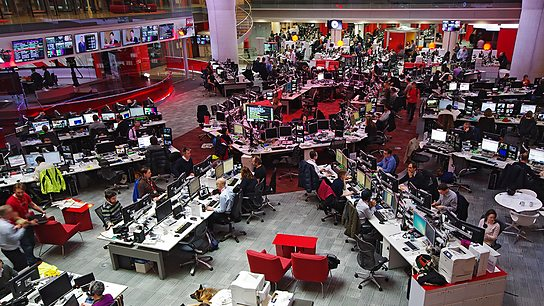
\includegraphics[width=\columnwidth]{figs/newsroom.jpg}
  \caption{The newsroom in BBC New Broadcasting House.}
  \label{fig:newsroom}
\end{figure}

\begin{figure}[p]
	\centering
	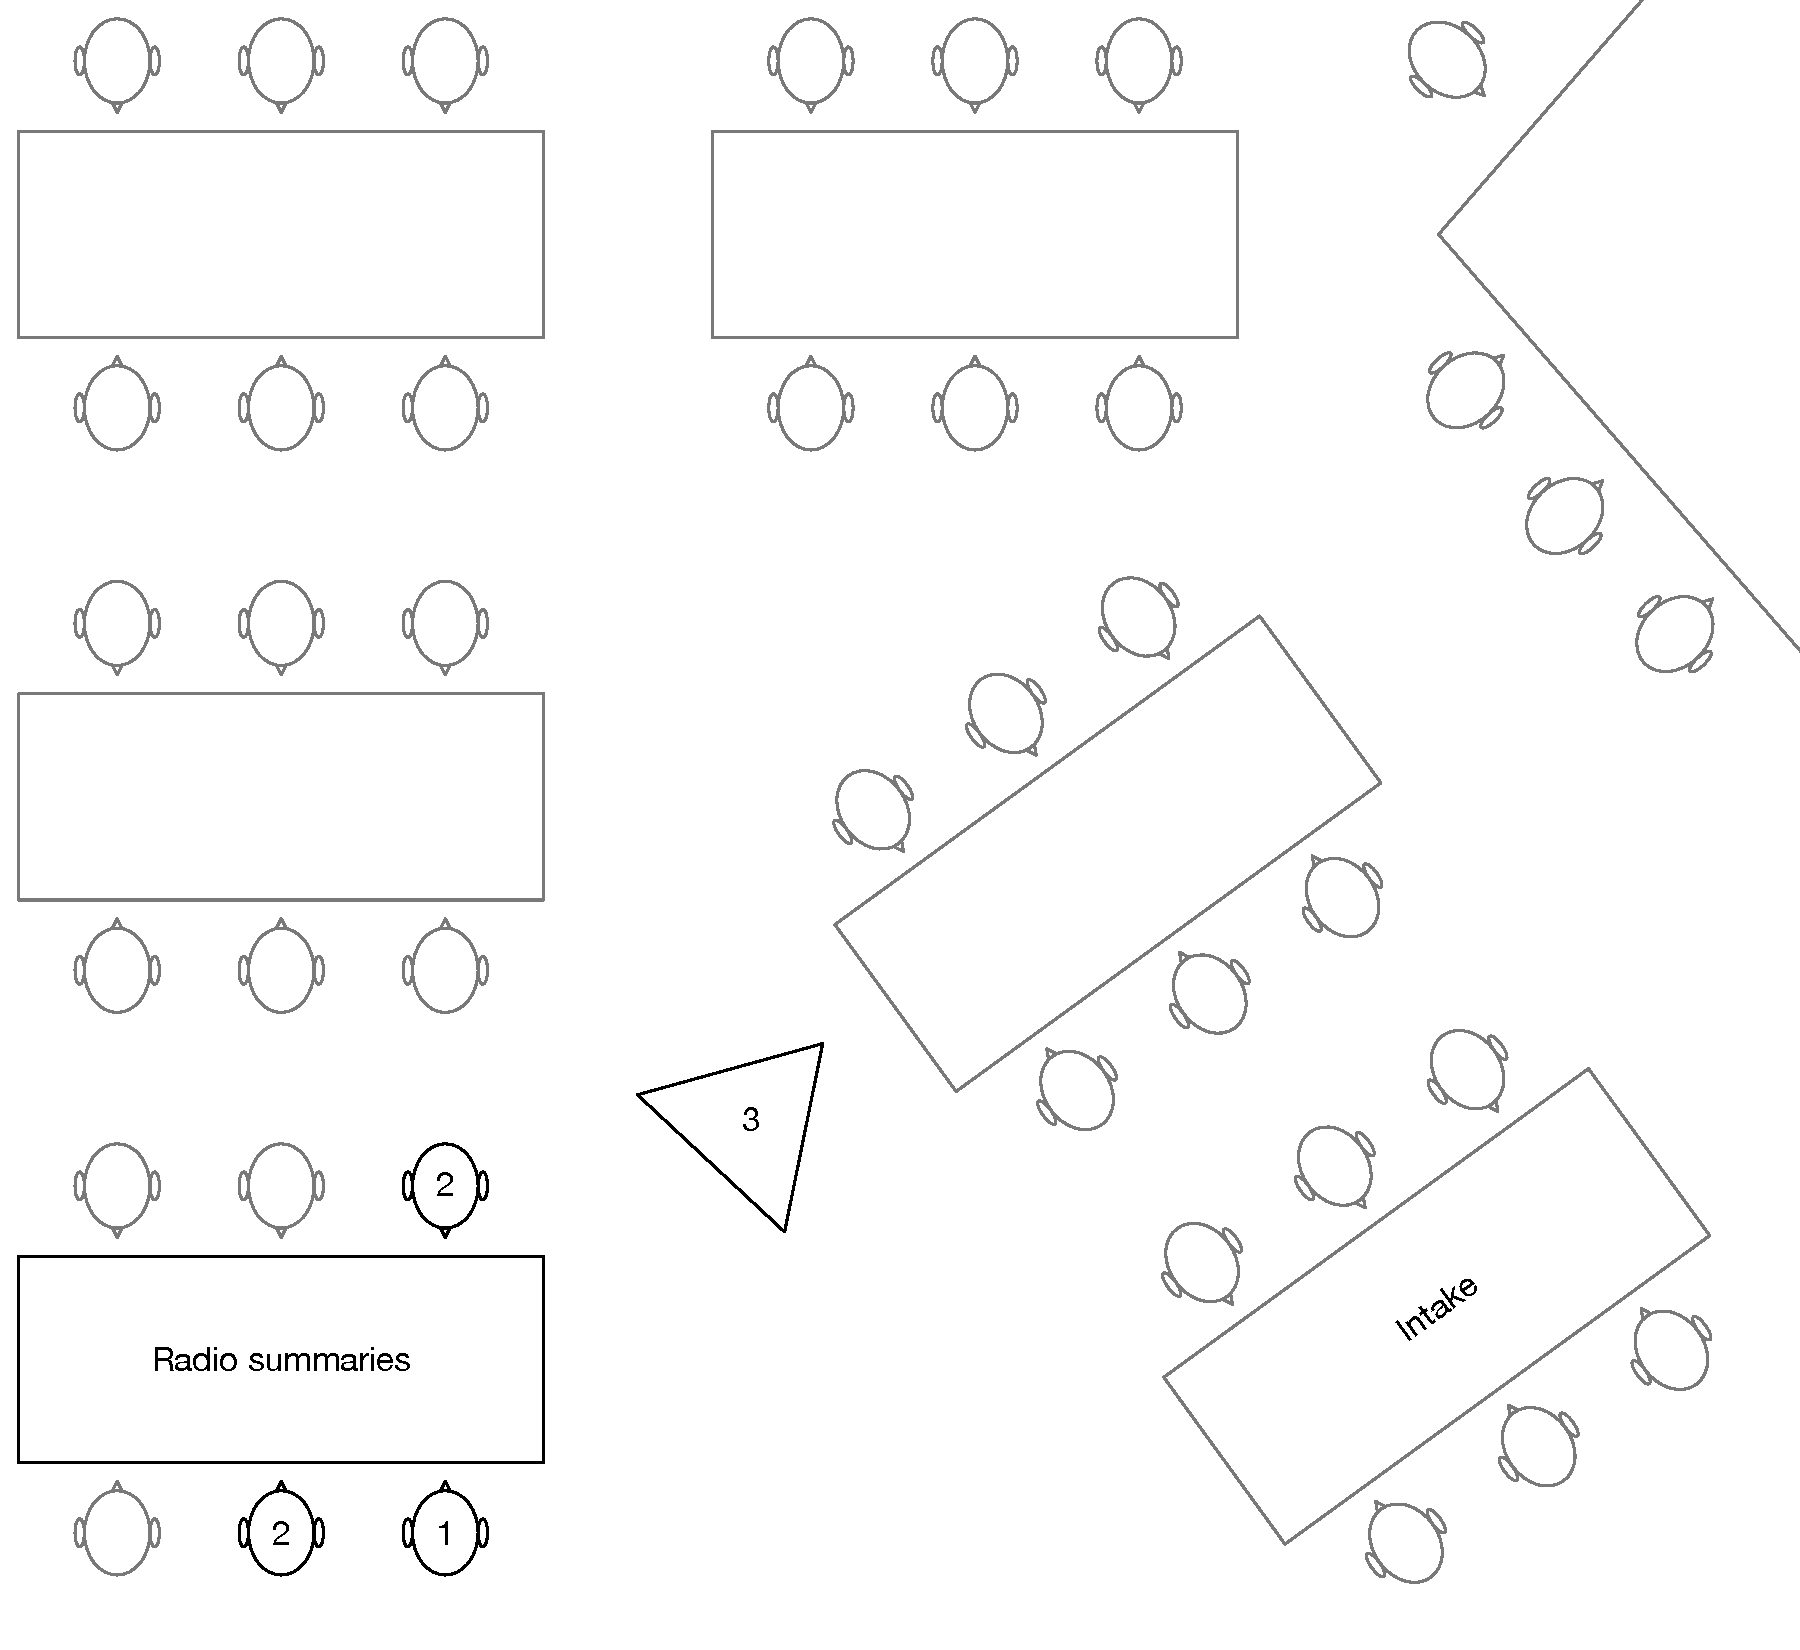
\includegraphics[width=4in]{figs/news-layout.pdf}
  \caption{Layout of radio summaries within the BBC newsfloor, showing the assistant editor (1), broadcast journalists
  (2) and the arrivals board (3).}
	\label{fig:newsroom-layout}
\end{figure}

\begin{figure}[p]
  \centering
  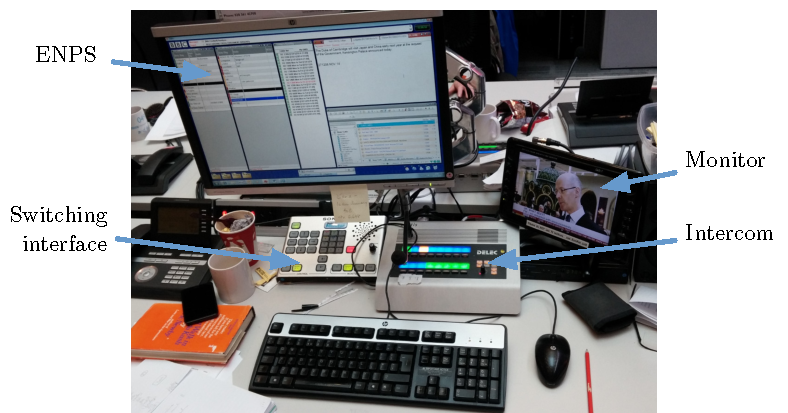
\includegraphics[width=\columnwidth]{figs/news-desk-labelled.pdf}
  \caption{Desk of the radio summaries assistant editor, showing ENPS (1), a switching interface (2) for controlling
  the output of a desktop TV monitor (4) and headphones, and an intercom (3) for communicating with other teams.}
  \label{fig:news-desktop}
\end{figure}

\begin{figure}[p]
  \centering
  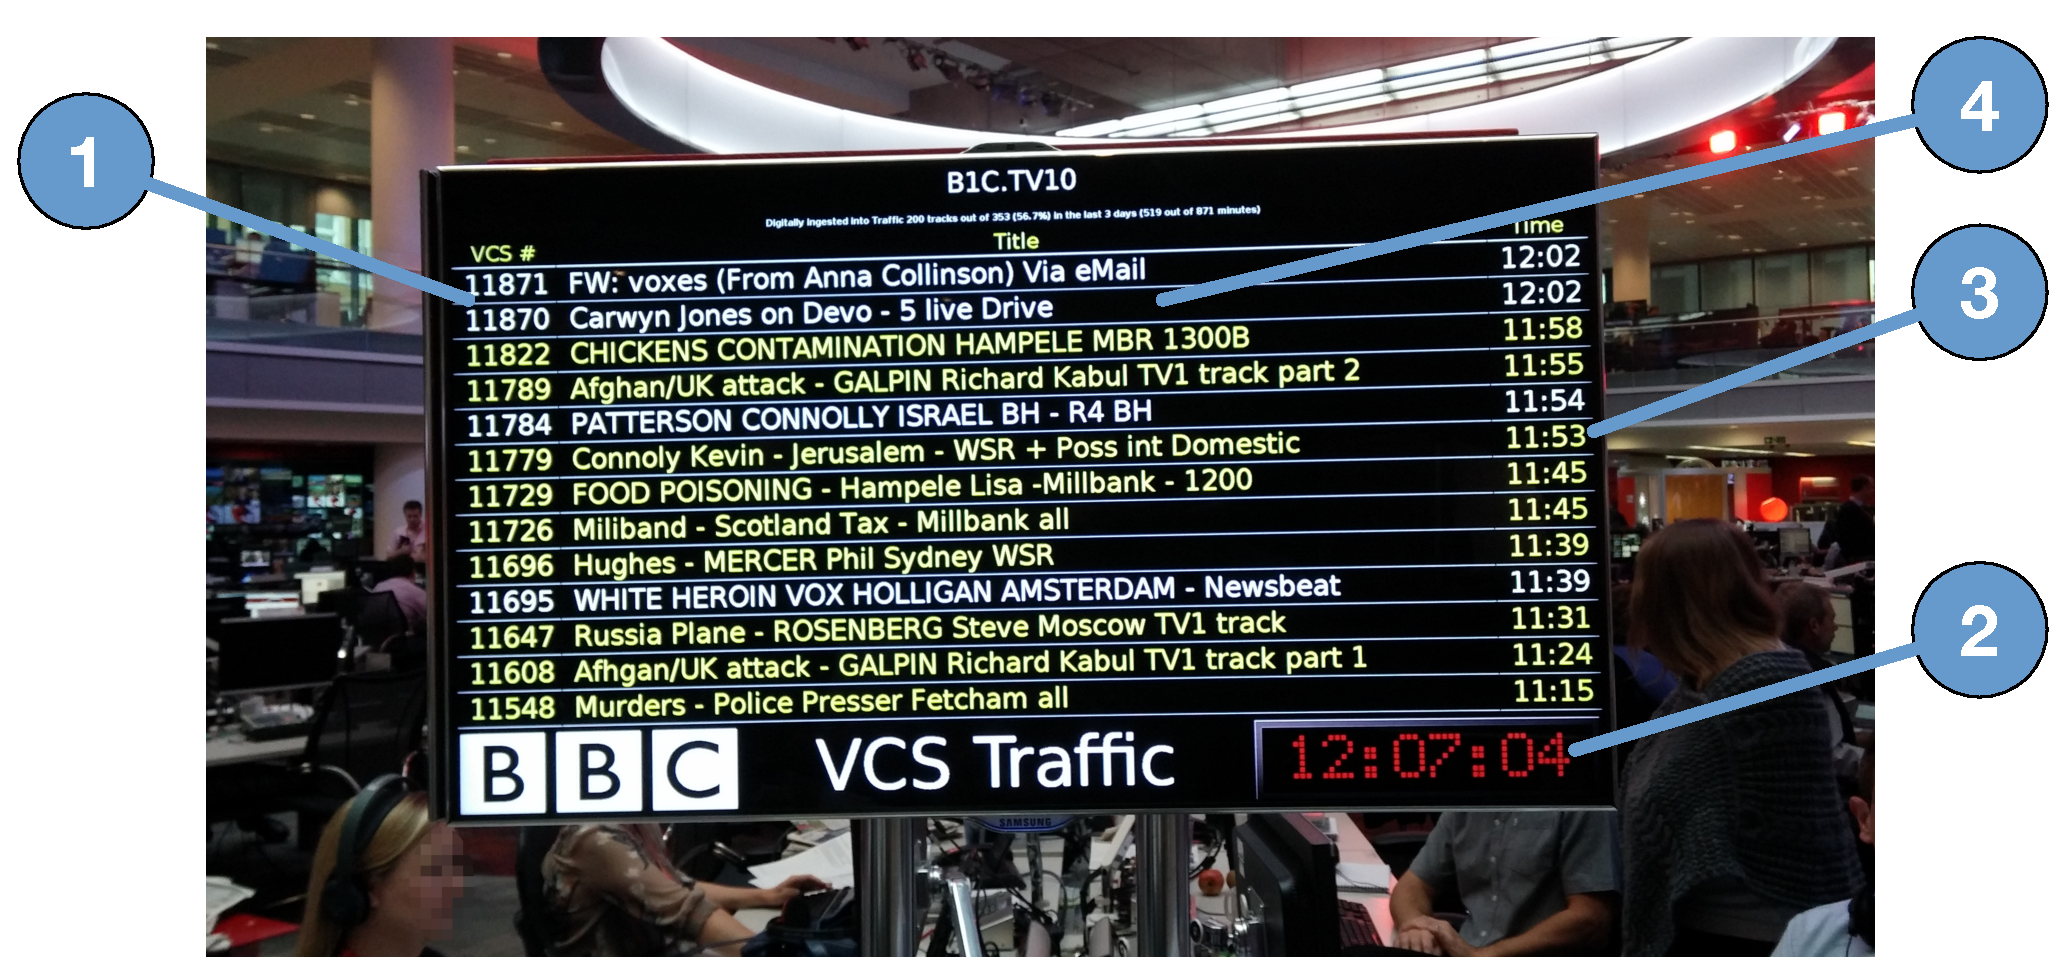
\includegraphics[width=\columnwidth]{figs/arrivals-board-labelled.pdf}
  \caption{Arrivals board in BBC newsroom, showing the ID number (1), arrival time (3) and name (4) of each audio clip.
  The screen also includes a clock (2). ``VCS'' is the colloquial name for the \textit{dira!} radio production system,
  as it is made by a company that used to be called VCS.}
  \label{fig:news-arrivals}
\end{figure}

The broadcast journalists and assistant editor write the summaries on a desktop PC using a software package called
``Electronic News Production System'' (\textit{ENPS}). Figure~\ref{fig:news-enps-edit} shows the ENPS interface. ENPS
is used for writing scripts, compiling and approving news bulletins, and monitoring newswire services\footnote{News
reports provided by global news agencies, such as Reuters and Associated Press}. The system is networked so that any
changes made in ENPS are instantaneously updated for everybody. Audio clips are browsed, imported and edited using a
plugin called Media Object Server (\textit{MOS}), which integrates with the \textit{dira!} radio production system.

\begin{figure}[ht]
  \centering
  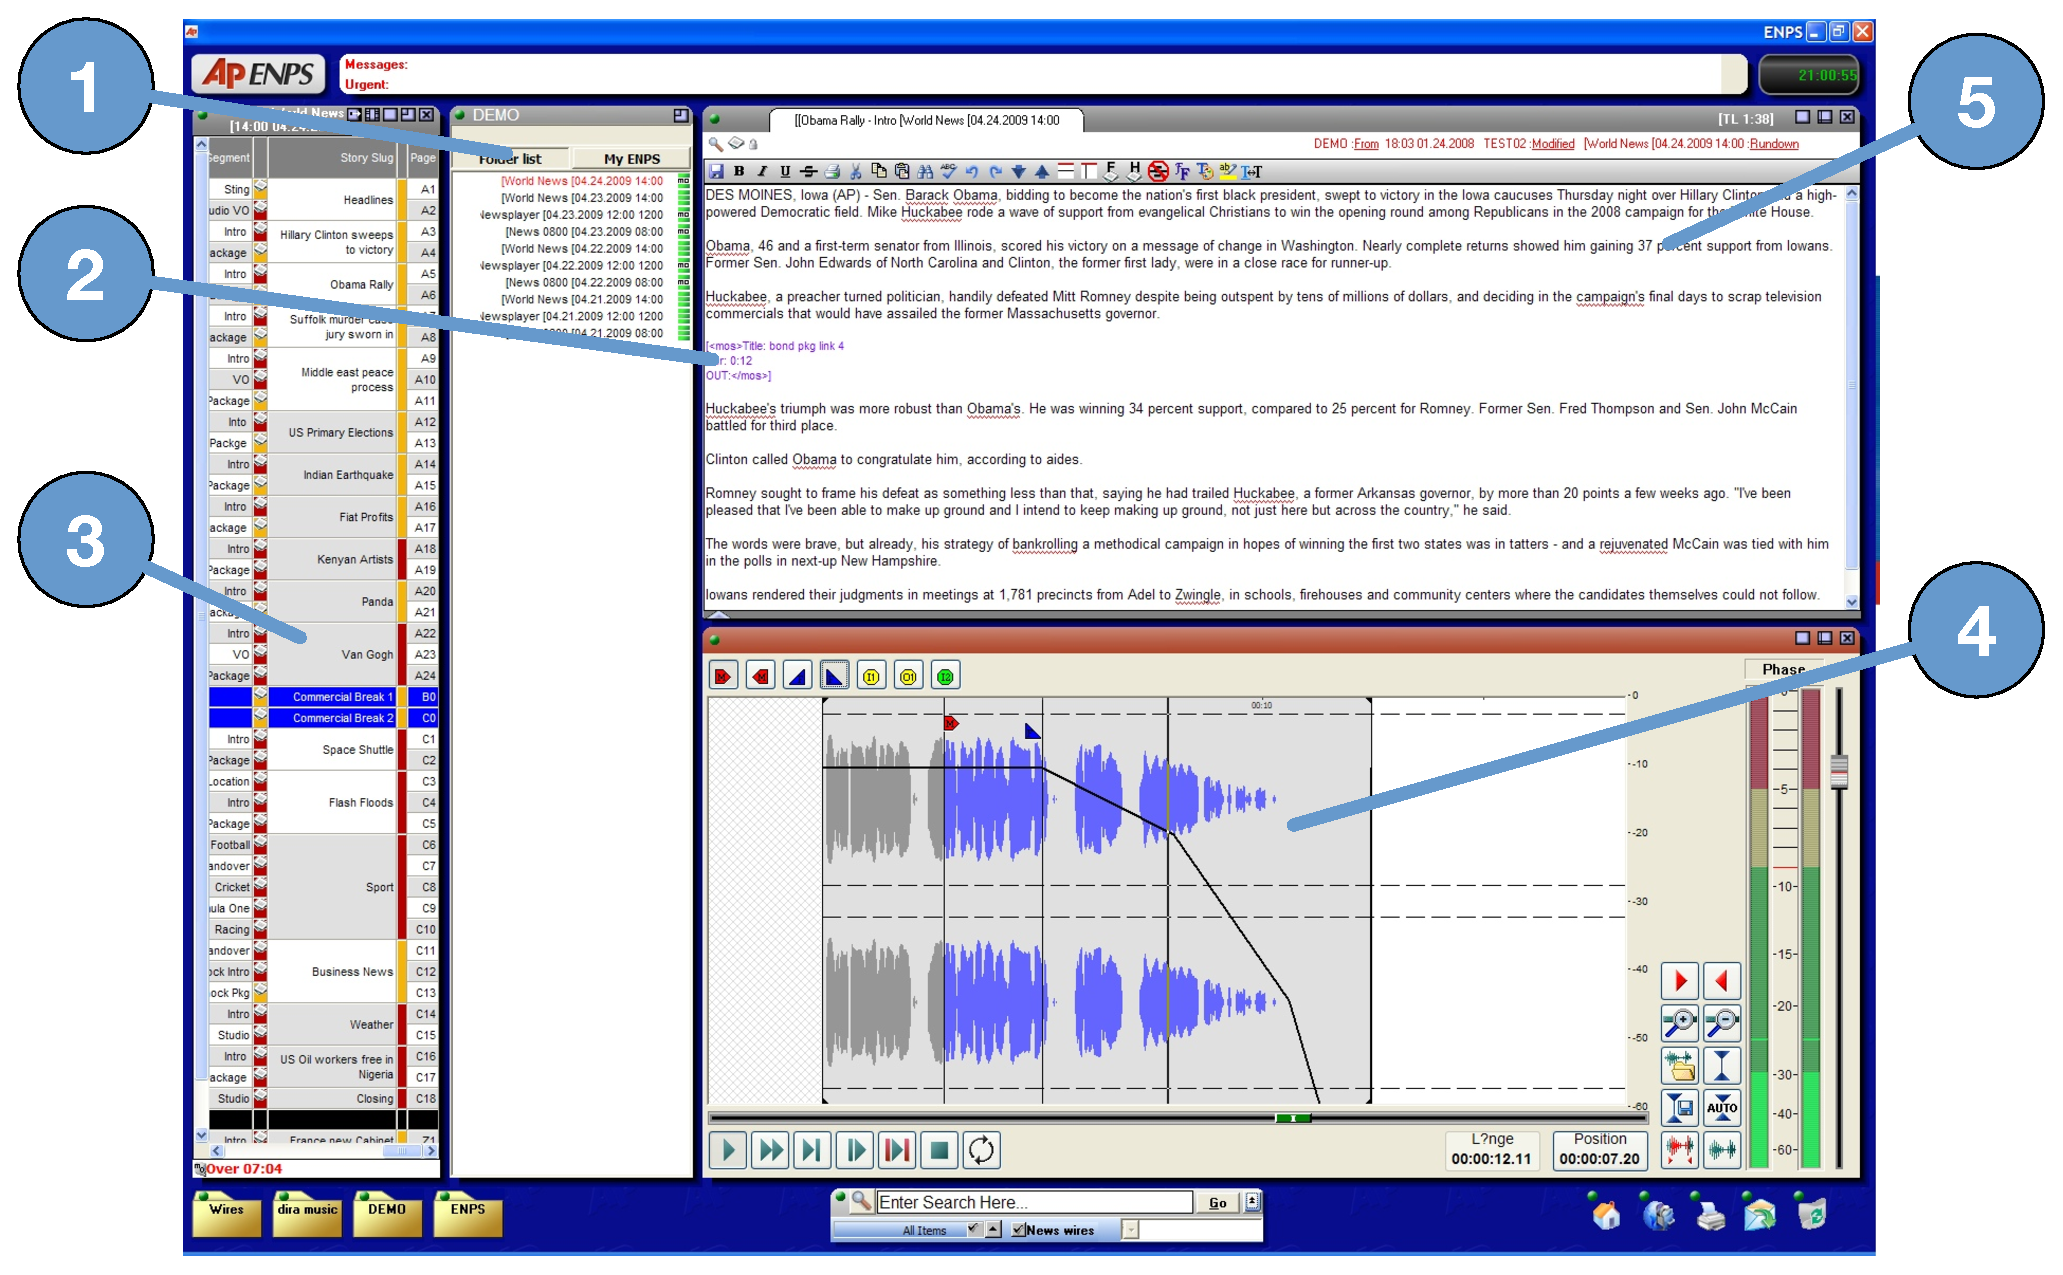
\includegraphics[width=\columnwidth]{figs/news-enps-labelled.pdf}
  \caption{Editing a clip in ENPS, showing the schedule and approval status of the news report (3), the list of drafts
  for each summary (1), the text of the summary currently being edited (5), audio clips inserted into the summary (2),
  and the ``MOS'' plugin for finding and editing audio clips in the \textit{dira!} radio production system}
  \label{fig:news-enps-edit}
\end{figure}

\subsubsection{Task analysis}
Figure~\ref{fig:news-flowchart} shows the operational sequence diagram of the radio summaries production process. A
description of the workflow is written below.

\begin{figure}[ht]
	\centering
	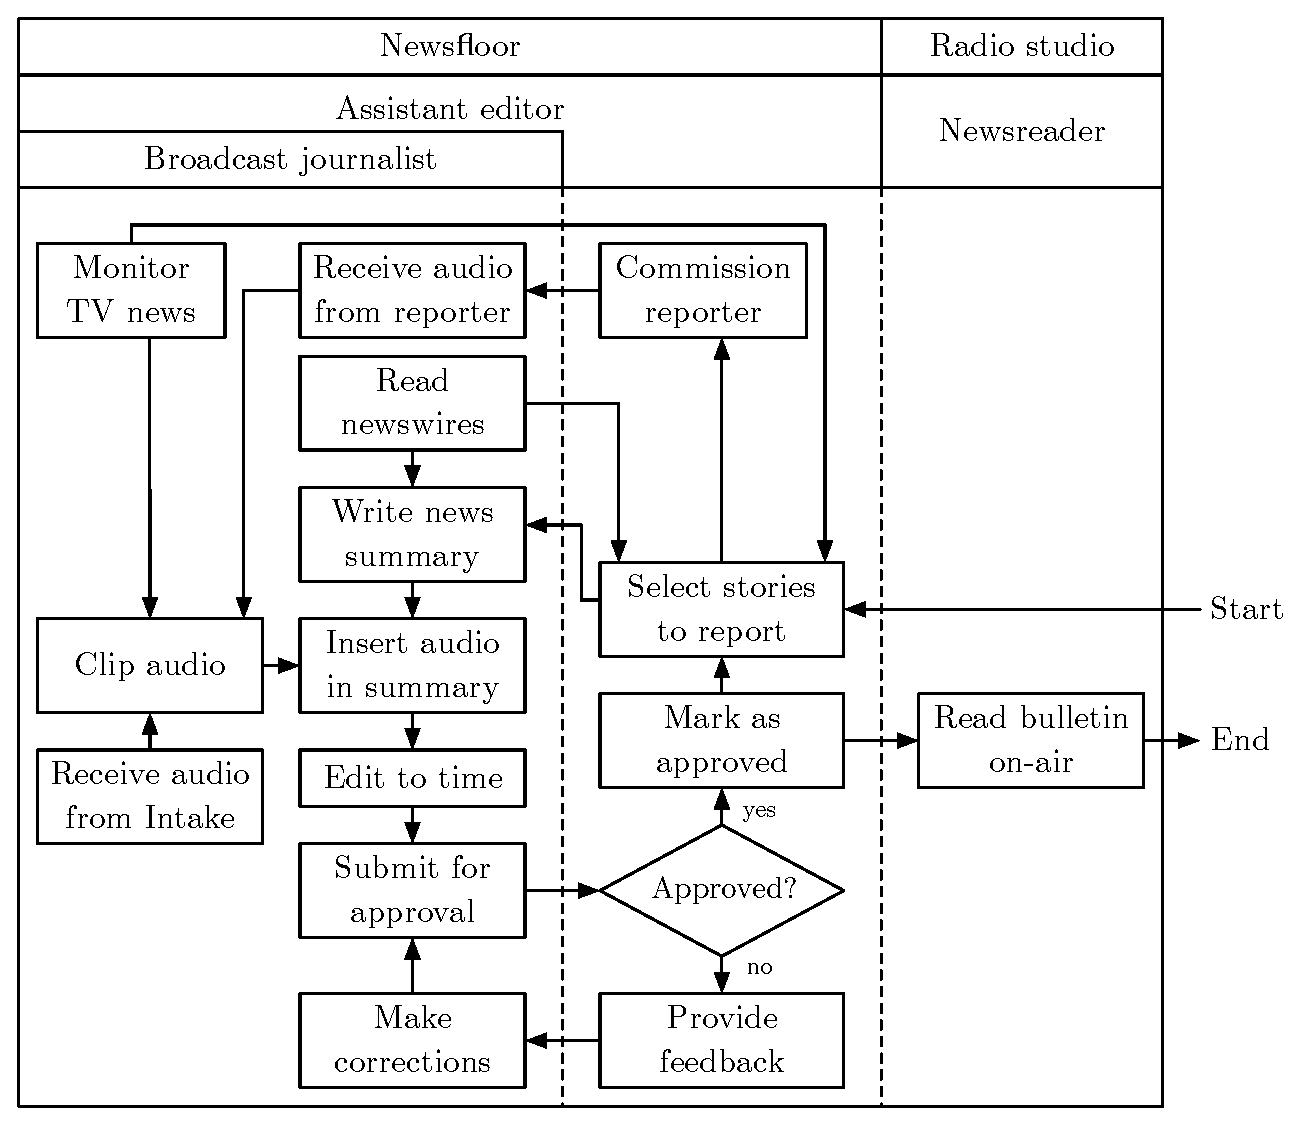
\includegraphics[width=4in]{figs/news-workflow.pdf}
  \caption{Operational sequence diagram of news summaries production, partitioned by role and location.}
	\label{fig:news-flowchart}
\end{figure}

% read newswires
% monitor TV news
% select stories
% commission reporter
% write summary
The assistant editor selects which news stories should be included in the bulletins. The stories come from multiple
sources, including newswire services and the BBC television news channel.  Newswire services are global news agencies
that provide news reports to subscribing news organisations, such as Reuters and Associated Press (AP).  Newswire
reports are accessed through ENPS, and users are notified of any reports flagged as important.  As they work, the
assistant editor and broadcast journalists keeps an eye on the BBC News TV channel using a small monitor on their desk.
They watch the channel to spot any breaking news stories, or material which they could use in their bulletins, such as
interviews.  The assistant editor will sometimes commission a reporter to record a news report for a particular story,
so that they have some quality audio content to include in the summary. The broadcast journalists and assistant editor
both write the summaries for a specific bulletin using ENPS. Previously-written summaries are often re-used, but are
updated to reflect the latest information.

% receive audio from reporter
% receive audio from intake
% monitor TV news
% clip audio
% insert audio
Audio clips are added to each summary to include quotes from interviews and items from reporters. The audio is sourced
from the Intake team, directly from reporters and from the BBC News TV channel. Audio from Intake and reporters is
imported using the \textit{MOS} plugin. This allows users to find audio in the \textit{dira!} radio production system
and edit clips by cutting the audio, and controlling sound levels/fading. Finished clips are inserted directly into the
text of the written summary using a drag-and-drop gesture. At this point, the broadcast journalist gives the clip a
name and can optionally include the ``in/out words'' that are spoken at the start and end of the clip.  The name,
in/out words and duration of the clip appear in the script.  Audio from the BBC News TV channel must be found and
clipped by the broadcast journalist themselves. The sound from the televison channel is automatically recorded into
\textit{dira!} in 40-minute segments. The broadcast journalist uses the \textit{MOS} plugin to browse to the desired
segment, find the location of the audio they want, and create a clip of the audio.

% edit to time
% submit for approval
% provide feedback
% make corrections
% read bulletin on-air
The finished bulletin must fit an exact time slot (e.g. two minutes), so the broadcast journalist must estimate how
long it takes to read their bulletin and edit the text to the correct length.  When a journalist has finished writing
their bulletin, it is placed into the `running order' and named according to the network and time (e.g. `R4 Thu
10:00').  The assistant editor then reviews the bulletin and listens to the clips. This is to ensure the bulletin is of
the right length, is factually accurate, uses the correct language, and complies with BBC editorial policy and Any
required changes are made either by giving feedback to the journalist, or by the assistant editor making the changes
themselves.  When the item is approved in ENPS, it is labelled with a green flag, which indicates that it has been
signed-off.

The newsreader sits in a radio studio and normally has no direct contact with the summaries team.  At the time of the
news bulletin, the newsreader reads the script directly from ENPS while on-air. The audio clips in the script are
automatically loaded into the play-out system, and the newsreader uses a button to trigger them at the right time.  The
duration and in/out words of the audio clip are displayed in the script, which helps the newsreader to predict when the
clip ends.

\subsubsection{Challenges}

The summaries team work under high-pressure circumstances. They have less than an hour to put together several minutes
of content that will be read to millions of listeners. News can break at any moment, so sometimes bulletins need to be
changed or re-written minutes before they are broadcast. In addition to these pressures, it is very important that the
news reports are factually accurate and balanced.  Due to these circumstances, the particiants had very little time to
talk to the researcher. During observation, all of the communication between team members was directly related to the
task at hand, and there was no chatting or socialising.

When creating clips from television broadcasts, the broadcast journalists must source the clips from 40-minute-long
segments.  To find the audio, they would seek through the recording, listening for a particular voice or mention of the
topic of interest.  The \textit{MOS} plugin interface they used displayed a waveform, but this did not seem to help
them find the audio.  This made finding and cutting clips a time-consuming and difficult task, particularly when
performed under pressure.  Application of segmentation or speech-to-text technology could help by indicating where
people are speaking, displaying keywords that are mentioned, or allowing the recording to be searched by text.

The bulletins written by the broadcast journalists must target a specific duration for when they are broadcast. It is
difficult for them to write and edit the script so that it contains all the facts, is balanced and reads well while
hitting the correct duration. However, in addition to this, they have no indication of how long it takes to read a
piece of text. They must therefore estimate this based on experience, or reading it in their head.
By developing a system that estimates the duration of spoken text, broadcast journalists may be able to target a
specific duration more efficiently. 

When it comes to inserting clips into the script, in and out words must be manually entered so that the clip can be
recognised, but there is not enough time to transcribe the whole clip.  Speech-to-text technology would be able to
automate this and full transcription could further help the journalists to recall the clip and write the script around
it.

\subsection{Drama}\label{sec:drama}
Radio 4's ``15 Minute Drama'' is a series of original drama and book dramatisations, broadcast twice-daily. Production
of drama is very different from most other genres in radio, as it is based on a pre-written script of a radio play. The
drama is created over several weeks. The researcher observed the production over two full days -- one for the recording
of the drama and the other for the editing process.  The observation did not include the writing of the script.

\subsubsection{Roles and responsibilities}
The production team is led by a \textit{director} who works with a \textit{broadcast assistant} and three studio
managers (SMs) -- a \textit{panel SM}, \textit{grams SM} and \textit{spot SM}. The team record a \textit{cast} of
actors who perform the drama.

The director is responsible for leading the team and making editorial and creative decisions. Before the recording,
they will have commissioned a writer to create the script, and worked with them to refine it. During the recording,
they announce the start and end of takes, and give feedback to the cast about their performances.  They also work with
the SMs to ensure the drama has the right sound.

The director is supported by a broadcast assistant who handles much of the administrative work before and after the
recording, such as making copies of the script, booking the cast, producers and rooms, and processing payments.
During the recording, they annotate the script with detailed notes about the position and length of each take, and mark
any mistakes or re-takes.

The panel SM is responsible for the sound of the drama. They lead the other two SMs during the recording process and
operate the mixing desk in the cubicle. They work with the spot SM to position the actors and microphones to achieve
they sound they want. They also make a backup recording of each performance onto CDs. After the recording, they work
with the director to edit the drama into the final version.

The grams SM prepares and plays pre-recorded sound effects during the recording, and is also responsible for recording
the performances using a DAW.  ``Grams'' refers to gramophones, which were historically used to play pre-recorded sound
effects.  After each take, the grams SM labels the recording with the episode, scene and take numbers, which are later
used to assemble the final programme.  When the director wants to listen back to a performance, the grams SM uses the
DAW to find and replay the desired take.

The spot SM works in the studio, rather than the cubicle, where they set up and position microphones and create spot
effects, also known as ``foley'' in the movie industry. The effects are produced using a large variety of props that
are kept in the studio to emulate common effects such as doors, windows, locks, telephones and footsteps to name a few.

The cast are hired by the director specifically for the drama being recorded. Often the cast are sourced from the BBC
Radio Drama Company (RDC), which is a rotating group of actors that are employed by the BBC. The cast perform the
radio play in the studio, working under instruction from the director.

\subsubsection{Environment and tools}
The drama we observed was recorded in Studio 60A, which is a purpose-built flexible performance space at BBC New
Broadcasting House in London. The studio contains spaces with different acoustic properties, including movable
absorbers and a foam-lined spiral corridor that used to simulate distance. There are many fixtures and props for
re-creating common environmental sounds including freestanding doors/windows with a variety of knockers and letter
boxes, a staircase with wood, concrete and carpet steps, an upstairs bedroom and a fully working kitchen.  In addition,
there are a wide range of props that are used to create spot effects.  The studio is a large space, so there are four
CCTV cameras which are used to allow the producers in the cubicle to see parts of the studio that are out of view. 

The studio is connected by a large acoustically-isolated window to the cubicle where the production team sit.
Figure~\ref{fig:drama-studio} shows the view of the studio from the cubicle, and Figure~\ref{fig:drama-layout} shows
the layout of the spaces. The mixing desk is operated by the panel SM and is positioned directly in front of the
window.  The broadcast assistant sits to the right of the panel SM and the director sits directly behind them. The
grams SM sits at the back of the room, while the spot SM spends most of their time in the studio.
%TODO Intercom

The panel SM sets the sound levels and balances the audio using the mixing desk, and makes a backup recording of the
performances using a CD recorder located in a rack to the left of the mixing desk.  Under the mixing desk, there is a
foot pedal which controls a light in the studio to silently indicate the start of a performance, known as a ``cue
light''. The panel SM also controls warning lights displayed above the door to the studio to stop people from walking
in mid-performance.  The grams SM uses software called ``SpotOn'' to select and play pre-recorded sound effects. They
use the ProTools DAW to record each performance, and label them with the episode, scene and take numbers.

Figure~\ref{fig:drama-edit} shows the editing suite where the panel SM and director perform the post-production work.
The editing suite is a compact acoustically-treated room which houses a PC running ProTools, stereo speakers, a small
mixing desk and level meters.  The left monitor is used to find pre-recorded sound effects and the right monitor is
used to arrange and edit the drama recordings. The panel SM uses an annotated copy of the script to guide their
editing.

\begin{figure}[p]
  \centering
  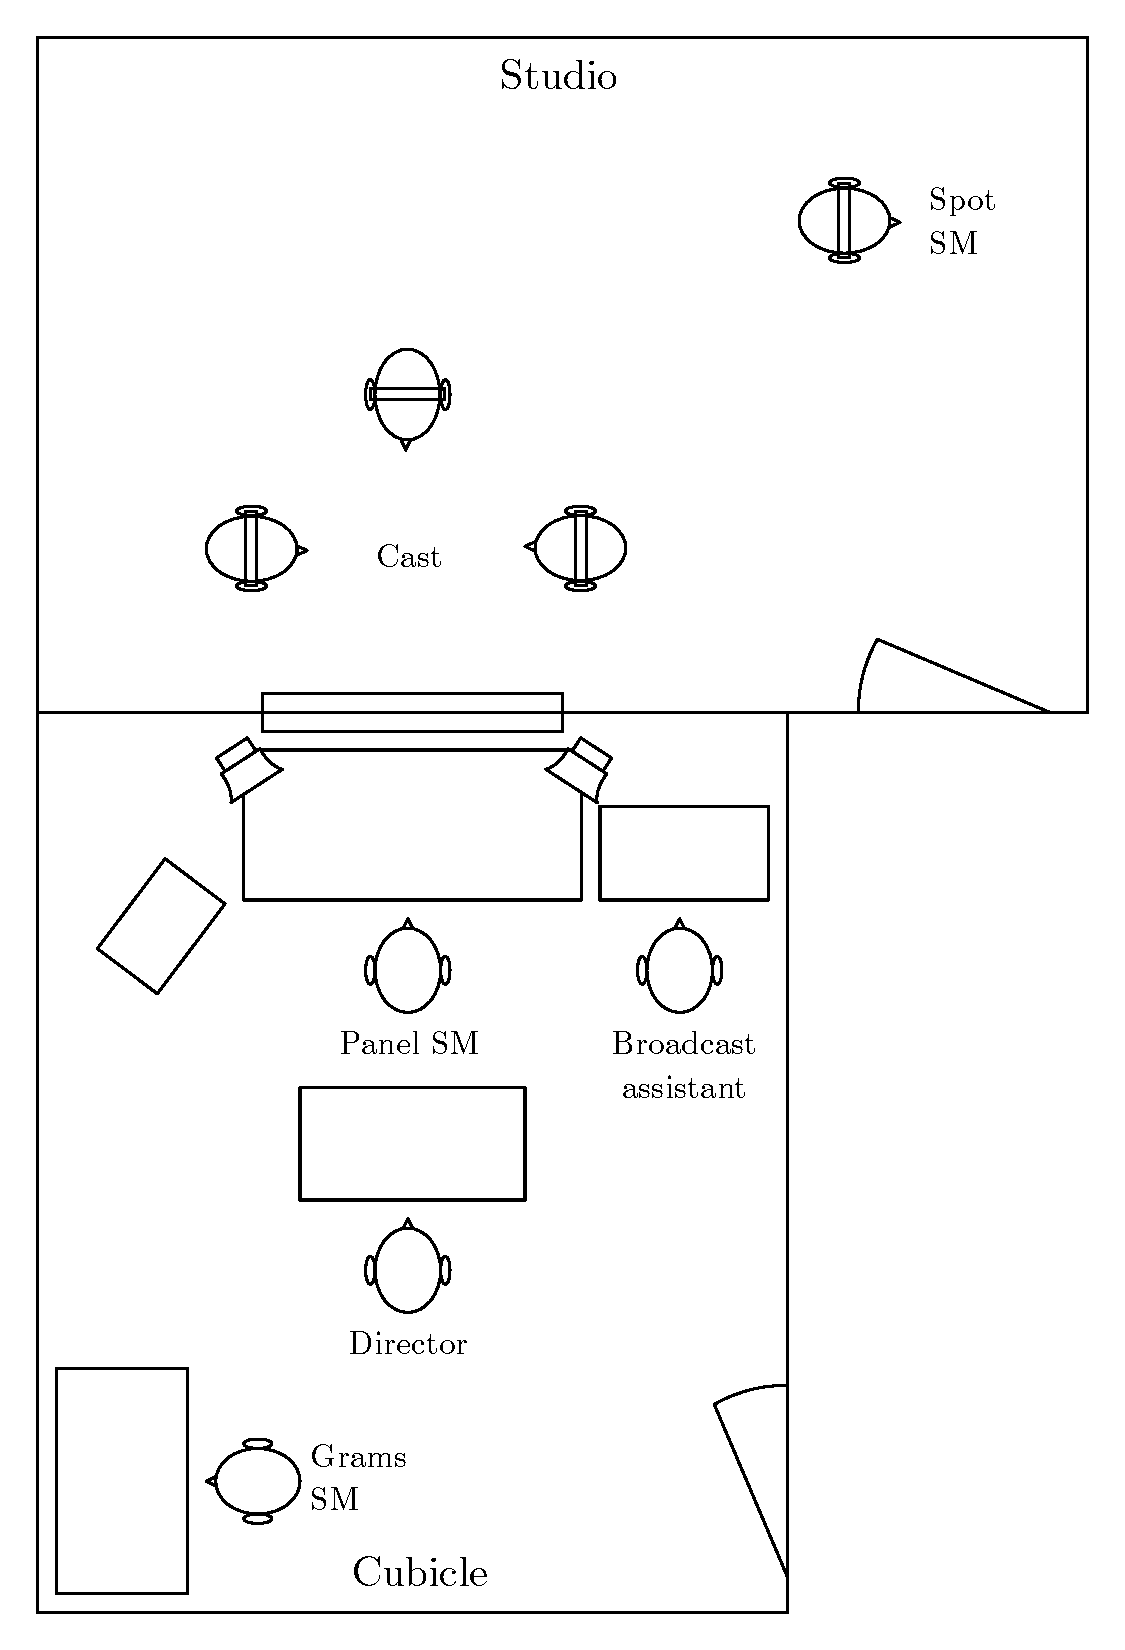
\includegraphics[width=3.5in]{figs/drama-layout.pdf}
  \caption{Physical layout of the drama studio and cubicle, showing the director (1), broadcast assistant (2), cast
  (3), panel SM (4), grams SM (5) and spot SM (6).}
  \label{fig:drama-layout}
\end{figure}

\begin{figure}[p]
  \centering
  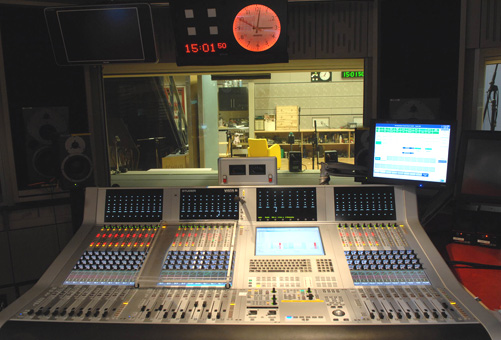
\includegraphics[width=\columnwidth]{figs/60a.jpg}
  \caption{Cubicle of studio 60A.}
  \label{fig:drama-studio}
\end{figure}

\begin{figure}[p]
  \centering
  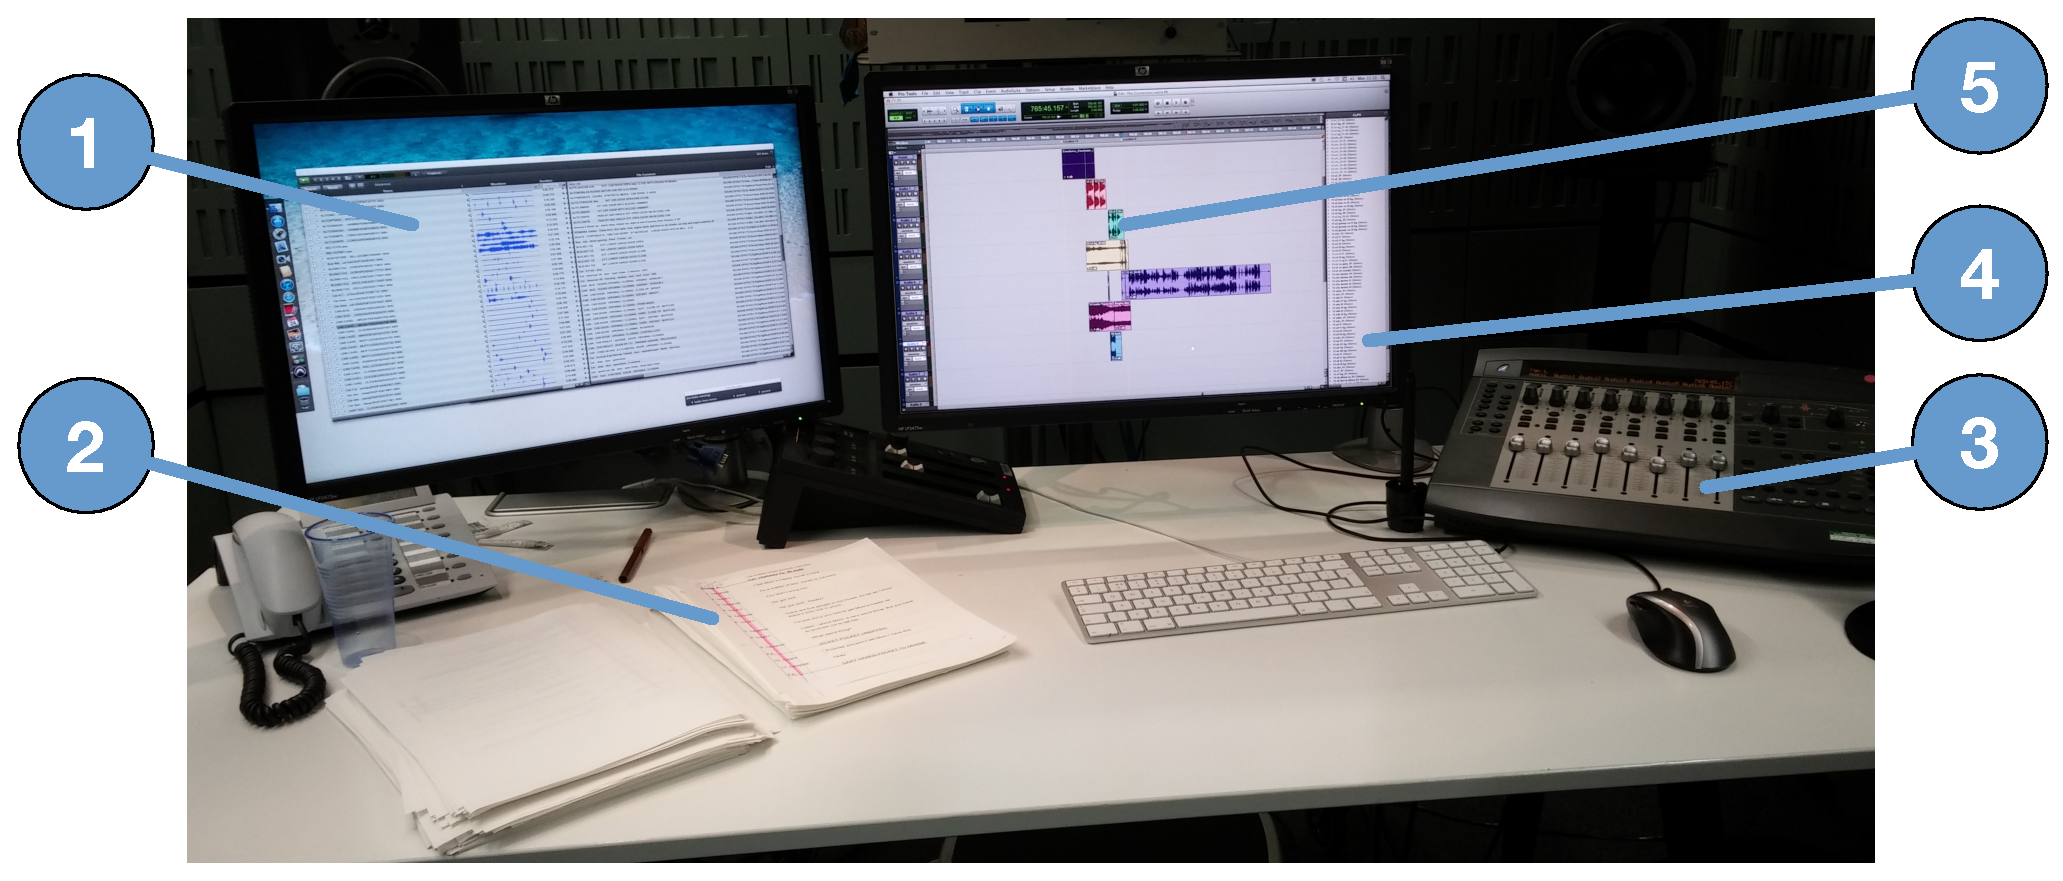
\includegraphics[width=\columnwidth]{figs/drama-edit-labelled.pdf}
  \caption{Radio drama edit suite, showing the sound effects library interface (1), the annotated script being edited
  (2), a mixing desk (3), the ProTools DAW with a list of recorded and labelled audio clips (4) and the edit time-line
  (5), and level meters (6).}
  \label{fig:drama-edit}
\end{figure}

\subsubsection{Task analysis}
Figures~\ref{fig:ethno-drama-recording} and \ref{fig:ethno-drama-editing} show the operational sequence diagrams of the
radio drama recording and editing process, respectively. Descriptions of each workflow are presented individually
below.

\begin{figure}[p]
  \centering
  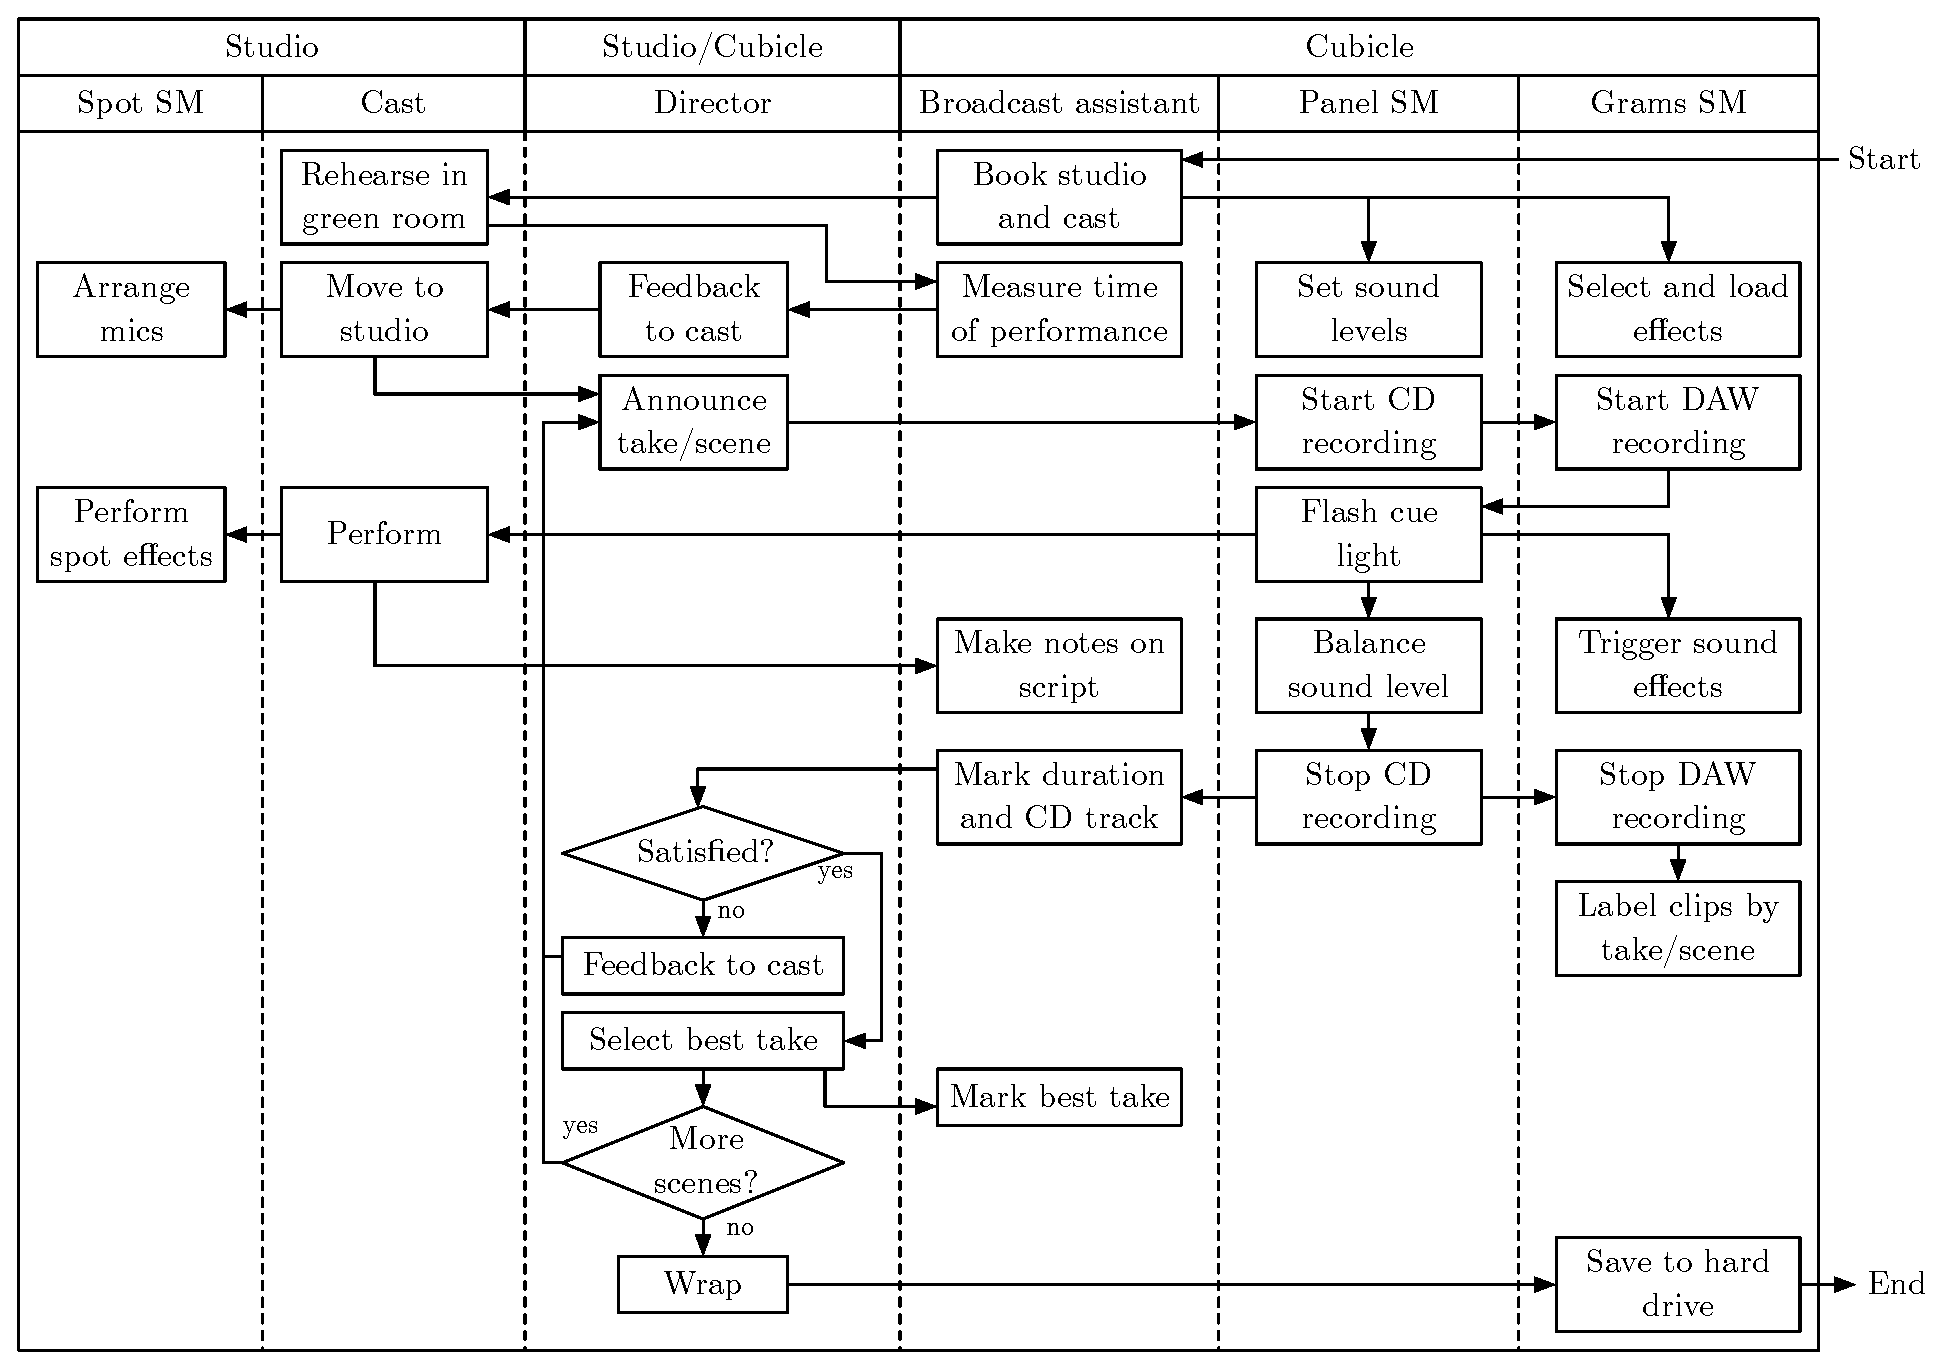
\includegraphics[width=5in]{figs/drama-recording-workflow.pdf}
  \caption{Operational sequence diagram of radio drama recording, partitioned by role and location.}
  \label{fig:ethno-drama-recording}
\end{figure}

\paragraph{Recording}
The recording process involves the entire production team and cast. Between one and two episodes are recorded in a day.
Prior to recording, the cast will assemble in the ``green room'' with the director and rehearse the play. During the
rehearsal, the broadcast assistant measures how long the performances take, to ensure they are not too long or too
short.  The director provides feedback to the cast on their performances before they move to the studio.

The drama is recorded as a series of ``takes''. Each take is a short segment of a scene in an episode, often only
20--30 seconds long.  Multiple takes of the same material are recorded so that the director can give feedback to the
cast on how they would like it to be performed.  The director starts the process by announcing the episode, scene and
take number.  The panel SM starts the backup recording, and the grams SM starts the DAW recording. When everything is
ready, the panel SM flashes the cue light, which signals the cast to start performing.  During each take, everybody 
listens to the performance. The panel SM balances the audio levels, the grams SM triggers pre-recorded sound effects,
and the spot SM performs live spot effects in the studio.

The broadcast assistant make notes on a spreadsheet about the takes and their duration. They also annotate a printed
script with information about each take.  Figure~\ref{fig:drama-script} shows an example of an annotated drama script.
The start and end of each take is marked with a vertical line on the side of the page. The take and backup CD numbers
are written at the top of each line, and the duration of the take is written at the bottom.  If the take starts again
during a recording, the line continues back to the top.  The best take for each scene is marked by highlighting the
line for that take.  Words that are spoken incorrectly are underlined, and repeated words or phrases are marked with
square brackets.  Different coloured pens are used to distinguish the marks for each take.  If multiple brackets
overlap, their order is labelled with numbers.

\begin{figure}[p]
  \centering
  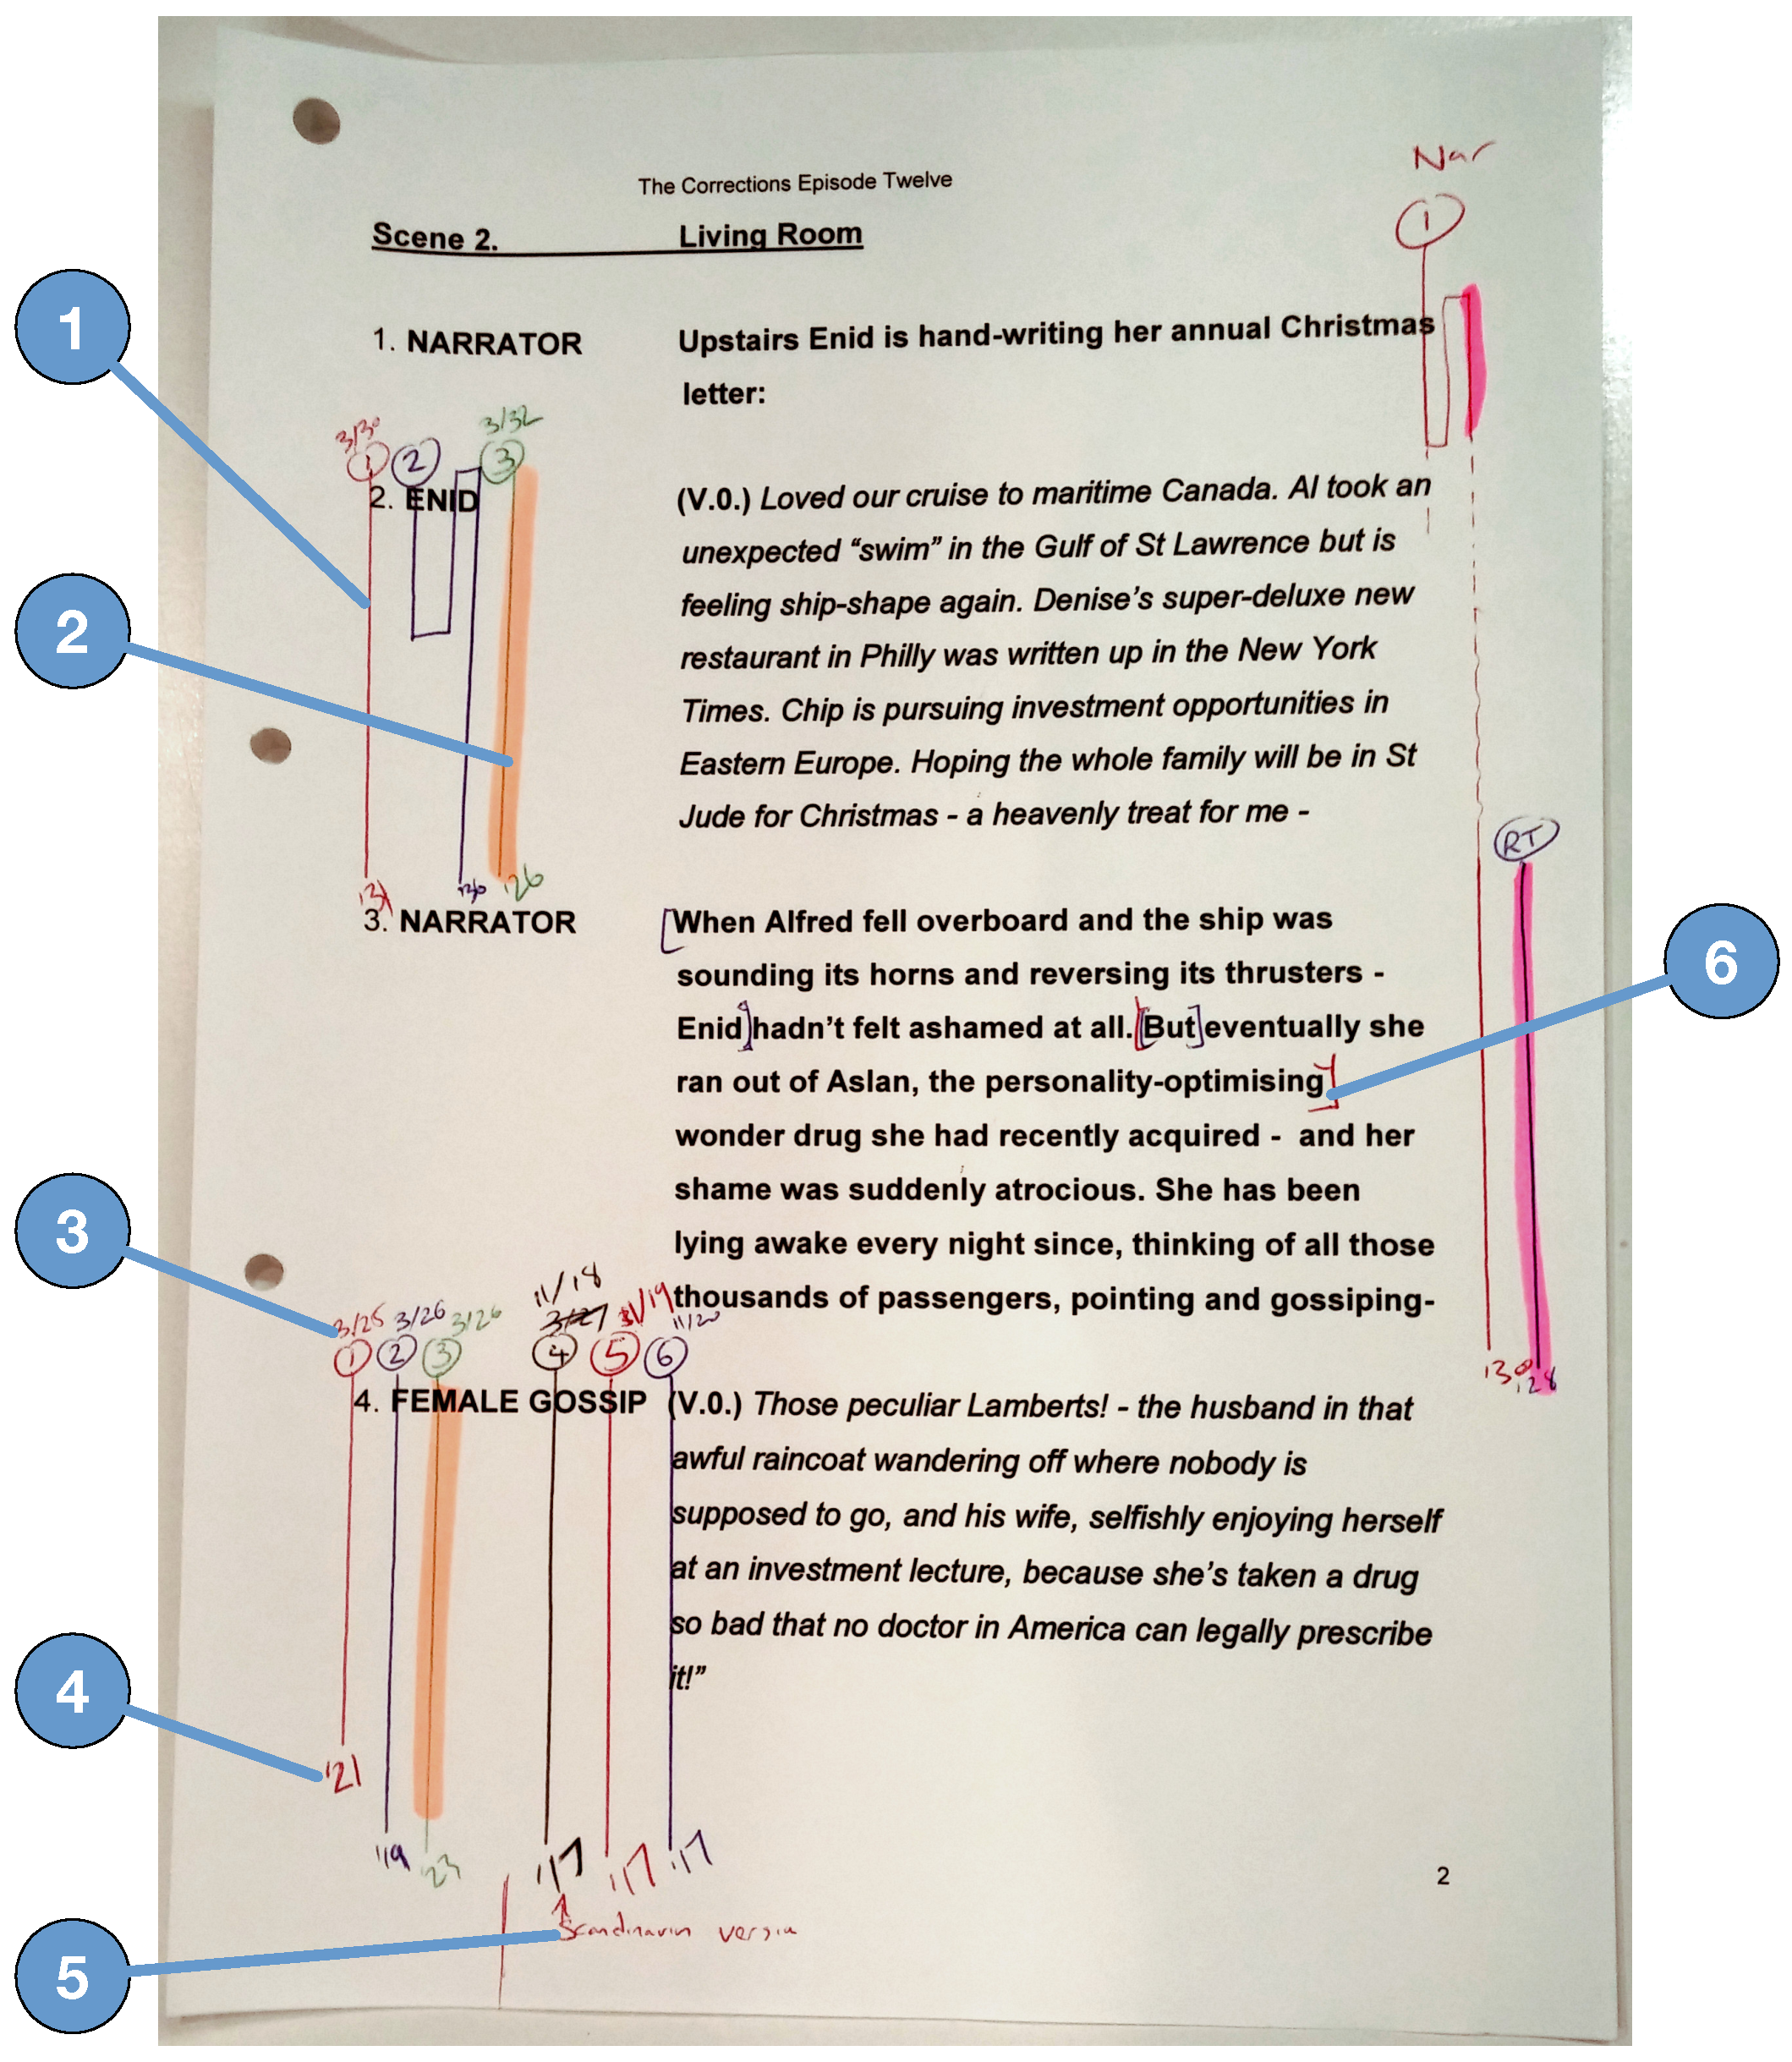
\includegraphics[width=\columnwidth]{figs/drama-markup-labelled.pdf}
  \caption{An annotated drama script page. Recordings for each take are marked with different colour lines (1). The
  best takes are marked with a highlighter pen (2). The backup CD and track number are marked at the top of each line
  (3) and the length of the take is marked at the bottom (4). Notes are often attached to takes (5). Repeated lines are
  marked using square brackets in the colour of the take (6).}
  \label{fig:drama-script}
\end{figure}

At the end of a take, the DAW and backup recordings are stopped. The grams SM uses the DAW to label the clip with the
episode, scene and take number (e.g. e2s3t1). The broadcast assistant marks the printed script and spreadsheet with the
duration of the take and the backup CD number.  If the director is satisfied that they have recorded what they need,
then they select the best take and move onto the next scene. The broadcast assistant marks the best take on the script
and spreadsheet. If the director wants to record another take, they discuss the performance with the production team,
then provide the cast with feedback, either by walking into the studio, or using the intercom.

When the recording is complete, the team either move onto a new episode, or the director sends everybody home.  The
grams SM copies the audio clips from the DAW onto a portable hard drive.  Portable hard drives are used as they can
handle large file sizes better than than the local computer network.  The portable hard drive and annotated drama
script are given to the panel SM.

\begin{figure}[ht]
  \centering
  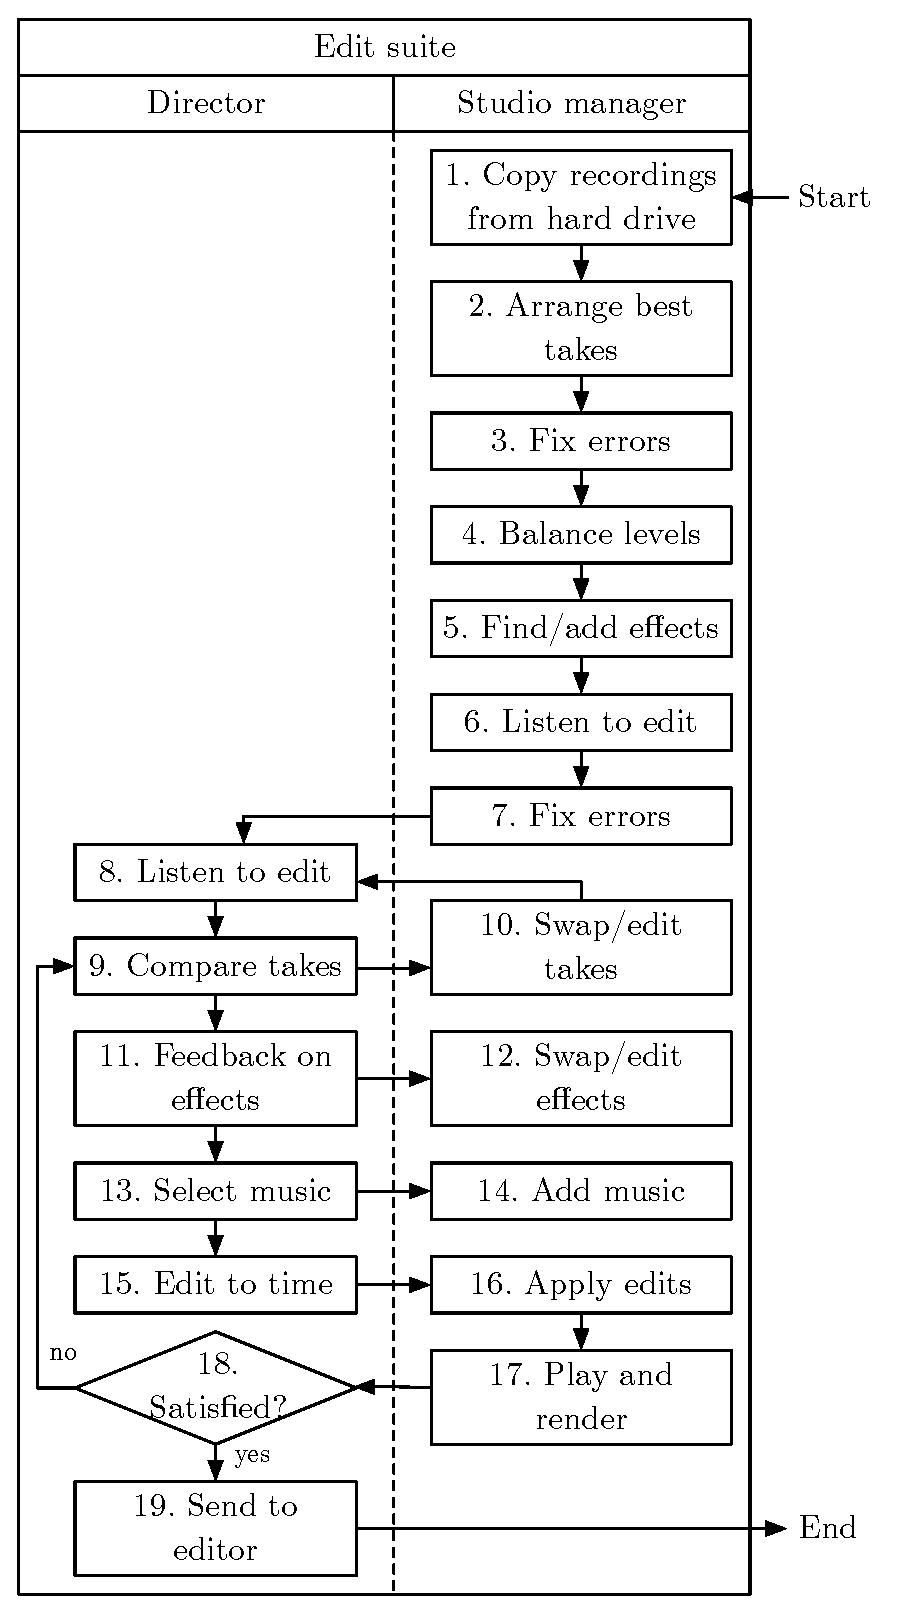
\includegraphics[width=2in]{figs/drama-editing-workflow.pdf}
  \caption{Operational sequence diagram of radio drama editing, partitioned by role and location.}
  \label{fig:ethno-drama-editing}
\end{figure}

\paragraph{Editing}
The recordings of the drama are edited into a final programme by the panel SM and director. The panel SM starts by
creating a rough edit of the programme by themselves, using the annotated script as a guide.  As the files are stored
on a portable hard drive, this process can be done either in an edit suite or on a laptop at home. The first step is to
create a sequence of the best takes from the recordings, as marked in the annotated script, by dragging them onto a
timeline from the list of labelled clips.  The panel SM uses the script to identify and remove errors in the takes,
such as re-takes or repeated words.  They adjust the sound level to be consistent throughout, either by using the mouse
to draw level curves, or by recording automation using a slider on the mixing desk.

The panel SM adds any sound effects that were not played at the time of recording using a sound effects library on
their PC, which contains roughly 900 hours of sound effects.  The effects are found either by using text to search the
metadata of the effects, or by browsing to a specific collections of effects.  Before the director joins them, the
panel SM listens through the rough edit to listen for any mistakes or errors, such as repeated words or phrases, or
noise caused by actors handling their paper scripts.  Double-speed playback is used to save time during this process.

Once the rough edit is complete, the director joins the panel SM in the edit suite. They will listen to the rough edit
to judge the quality of the performances selected as the best takes.  Often, the director will ask the panel SM to play
other takes so that they can compare them.  To do this, the SM finds the correct recording in the clip list, drag it
onto the timeline and find the correct position in the clip.  The director may ask the panel SM to swap a take, or
combine the start and end of different takes to use the best performances.  The same process happens for the sound
effects, which may be swapped or mixed together.

Music is not specified in the script, so the director has the freedom to choose what they want. Popular consumer music
services are used to find commercial tracks, but often directors will choose `production music', which is designed for
TV/radio and is easier to license. These can be searched using descriptive keywords using one of a number of online
music libraries such as Audio Network or Desktop Jukebox.  The director provides the music to the panel SM on a USB
storage device for them to insert and mix using the DAW.

The final programme must have an exact duration to fit its assigned broadcast slot. The programme is edited to be
slightly too long, so some lines have to be removed to reduce the programme length. Removing lines has a strong
editorial impact, so the director decides which lines to remove and the panel SM removes them using the DAW.  Once
finished, the final edit is rendered to an audio file by playing the programme through a digital loop-back. Although
this can be done faster, this playback forces the director and panel SM to listen to the programme from beginning to
end in one go. If they are happy with the edit, the director sends the file to their editor for sign-off and broadcast.

\subsubsection{Challenges}
The clear syntax used to annotate the drama script shows that the production workflow is well-organised and makes good
use of existing tools. However to convert those annotations into a rough edit stage, the SM must use a DAW to manually
arrange and edit the clips, and remove any marked errors. This can be a lengthy and tedious process. If the annotations
could be captured digitally, the rough edit stage could conceivably be fully or partly automated.

In addition to being script-based, a defining characteristic of drama production is that multiple takes are recorded in
order to capture the best possible performance. However, there is no simple way to directly compare performances. For
this reason, the director does not want to compare too many takes, and therefore relies heavily on the script
annotations and written notes. Providing a quick and easy method for the director to listen to and compare different
takes could potentially lead to selection of better performances.

When actors make a mistake, they often say the line again immediately. This is usually noticed and marked in the script
with square brackets. However, these can sometimes be missed and are not easy to spot using the DAW interface. 
Audio analysis techniques could be used to detect and highlight where this happens.

%It takes skill and experience to find the right sound effects
%know which words to use for the search or to know which CDs or collections
%to use for certain effects.

\subsection{Documentary}\label{sec:doc}
``The Report'' is a weekly investigative documentary that covers topical news stories. It is produced over a three week
period by the Radio Current Affairs department in BBC News and is broadcast at 8pm every Thursday on Radio 4. The
researcher observed the team for a total of four days -- one day during their research phase, one day during their
interviewing phase and two days during their editing phase.

\subsubsection{Roles and responsibilities}
The documentary is created by a team of three, made up of a \textit{producer}, \textit{presenter} and
\textit{researcher}.  At certain points during the production, the team is supported by an \textit{editor} and
a \textit{studio manager}.

The producer leads the team and makes the editorial decisions. They decide what the storyline will be, who to interview
and how the programme is edited together. They will pre-interview participants to screen them, record interviews with
them, transcribe recordings and create a rough edit of the programme.

The \textit{presenter} is a journalist who is the narrator for the documentary. They work closely with the producer to
craft the storyline, write the narrative, conduct interviews and edit the programme. The Report has a regular
presenter who typically works on two or three documentaries at once.

The \textit{researcher} assists the producer with research and investigation. They recruit for and set up interviews,
conduct pre-interviews, make recordings and transcribe them. 

The \textit{editor} leads the radio current affairs department. They do not participate directly in the production of
the documentary, but provide feedback to the team and give approval for the documentary to be broadcast.  Their
involement is limited to read-throughs and the sign-off.

The \textit{studio manager} (SM) joins the team on the final day of production to turn the producer's rough edit into
the finished programme. This process includes removing redundant speech, adjusting the pace of the speech, removing
unwanted noise and adding music.

\subsubsection{Environment and tools}
The team is based in BBC New Broadcasting House in London. Most of the work takes place in an open-plan office using
standard office desks with a PC and telephone. The research for the programme is desk-based and does not require any
special tools other than a web browser and telephone.  Face-to-face interviews are conducted either on-location, in the
office building or in a radio studio.  For interviews outside the studio, a portable audio recorder and microphone is
used to capture the audio.  Remote interviews are conducted by using a digital ``ISDN''\footnote{Integrated Services
Digital Network} link to a local radio studio, an IP-based link such as Skype, or over the telephone. The telephone is
always a last resort as it has the poorest sound quality.

The office is located directly beside four radio studios. The studios are organised into pairs so that one can be used
for recordings, with the other used as a cubicle. Each studio is acoustically treated and contains a PC with a DAW,
mixing desk, speakers, microphones and a telephone connected to a recorder. The studio is used to record remote and
face-to-face interviews and record the presenter's narration, listen to the programme and edit it into the final
version.

\subsubsection{Task analysis}
Figure~\ref{fig:ethno-docs-workflow} shows the operational sequence diagram of the documentary production.  A
description of the workflow is presented below.

\begin{figure}[ht]
  \centering
  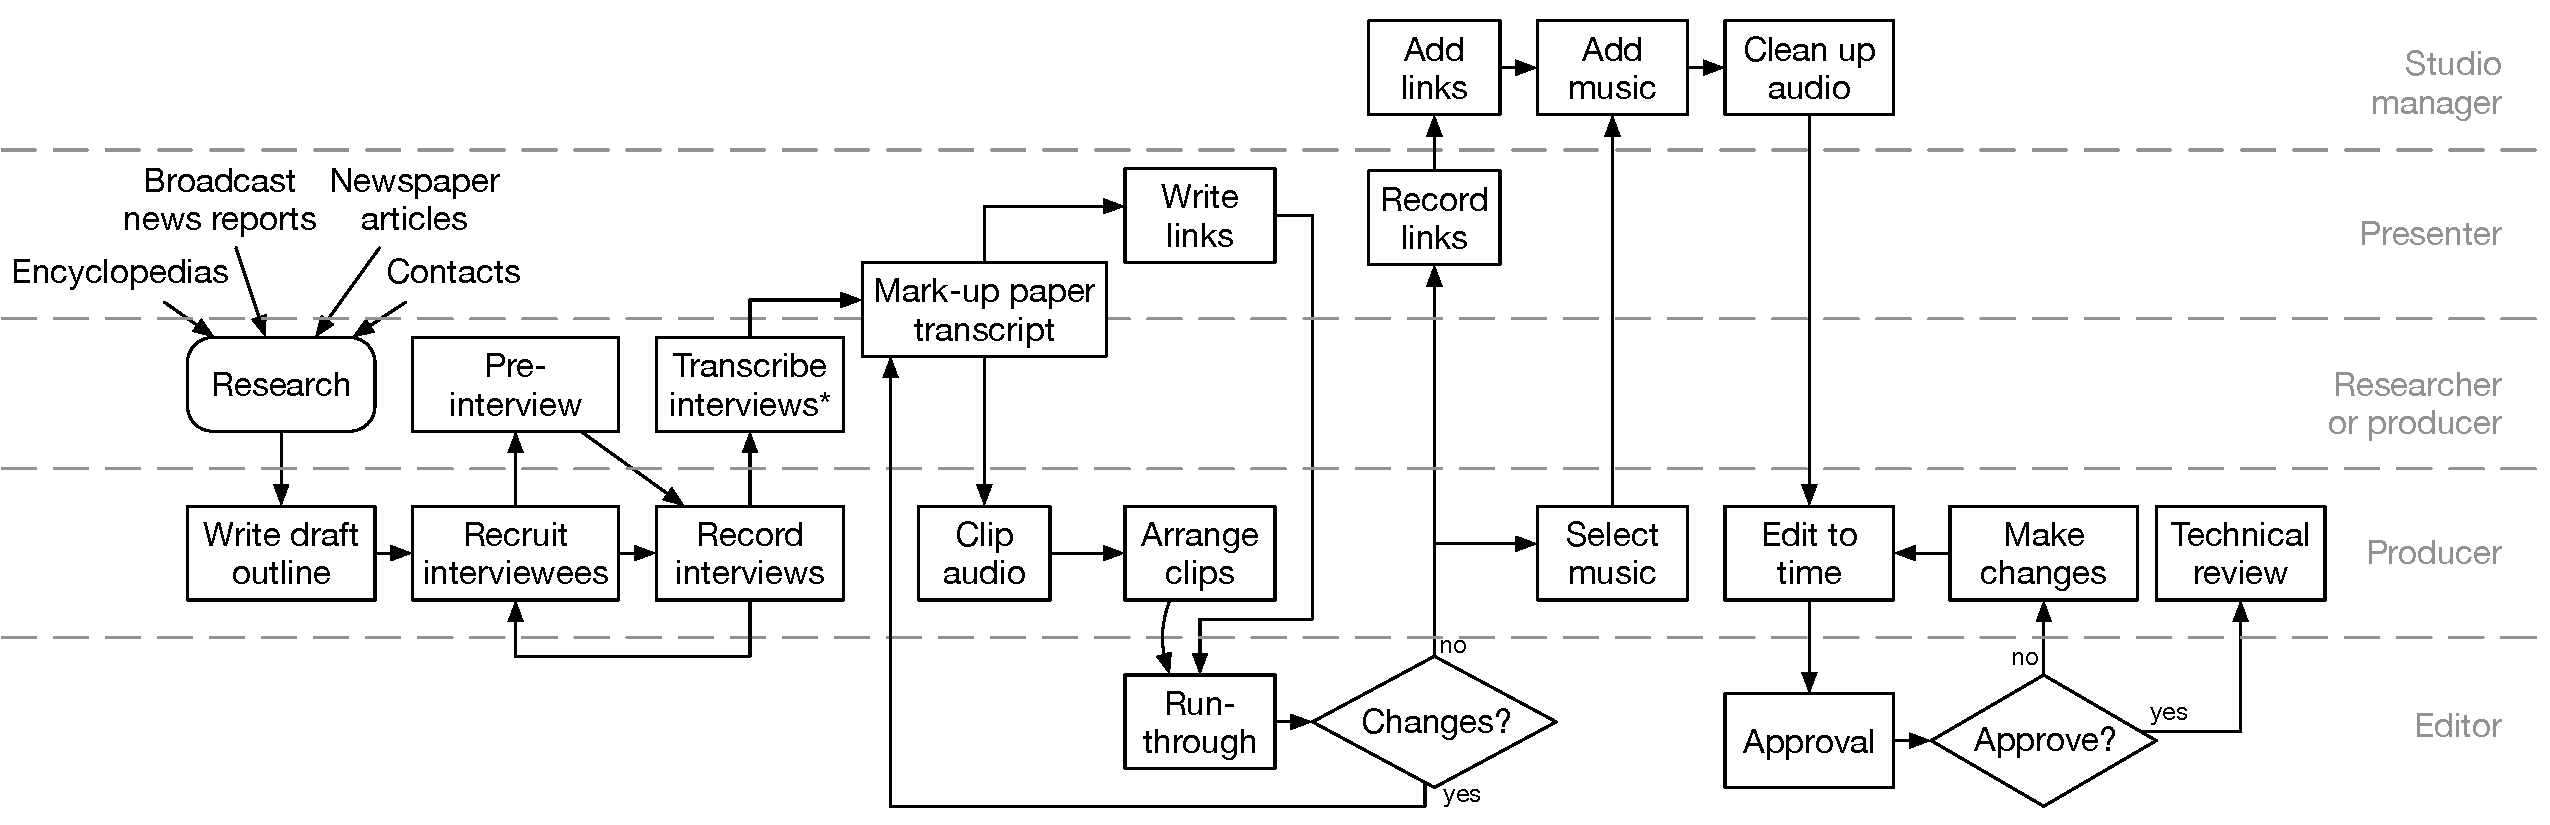
\includegraphics[width=4.5in]{figs/docs-workflow.pdf}
  \caption{Operational sequence diagram of radio documentary production, partitioned by role and location.\\
  {\footnotesize ($^{*}$some interviews are transcribed using a third-party service)}}
  \label{fig:ethno-docs-workflow}
\end{figure}

Production starts with researching the chosen topic of the documentary.  The purpose of the research stage is to form
the storyline for the documentary, and to identify people to interview.  Often the topic will be in the news that week
and the producer will be looking for an interesting angle which can be explored in greater depth.  The producer and
researcher listen to news reports and documentaries, read newspaper articles and encyclopedias, and talk to contacts
who know about the subject.  The producer makes rough notes for themselves in Microsoft Word and prepares a draft
outline of the programme.

Once the team have identified who they might want to interview, they will approach them to see if they are interested.
If the interviewee has the time available, the producer or researcher will do a `pre-interview' over the phone, which
simulates a real interview but is not recorded. This is done to see what the person will say and whether it suits the
storyline of the documentary.  Most interviews are recorded face-to-face, either on-location or in a studio, depending
on the situation.  During interviews, the presenter asks the questions while the producer records the audio and
monitors the levels.  For on-location interviews, the presenter holds the microphone and the producer operates the
portable recorder.

All of the interview recordings are transcribed. Some are recordings are sent to a third-party transcription service in
Australia that transcribes the audio overnight.  However, often the programme's budget can only cover transcription of
three or four interviews. The rest must be transcribed by the producer or researcher. For this, they use Microsoft Word
to manually type the transcript.  To save time, they will only do a rough transcription by skipping words, leaving only
enough to get a good idea of what they said.

The interview transcripts are printed onto paper, which the team use to help them collaborate.  The team go through the
interview transcripts and mark lines from they want to use with a highlighter pen. Notes and labels are informally
written on the page.  After the team have marked-up the interview transcripts, the producer uses them as a guide to
find the audio for the content they highlighted, and piece it together using a DAW into a rough edit. The transcripts
include timestamps every few minutes, which the producer can use to help them find the correct piece of audio.

While the producer creates a rough edit, the presenter writes the programme's `links' -- the narrative elements that
join the interview clips. When the first rough edit is complete, the whole team sits down with the editor for a
``run-through''. The programme is performed out loud from beginning to end, with the presenter reading the links and
the producer playing the clips from the DAW. This allows the editor to hear the programme and give early feedback. It
also allows the producer to determine the current length of the programme.  This run-through process typically happens
two or three times for each programme.

Once the editor is happy with the rough edit, a studio manager (SM) is brought it to help turn it into the final
programme.  This often happens on the day of the broadcast.  The SM records the presenter's links directly into the
DAW, while the producer sits in and gives feedback to the presenter.  The programme's theme music is added, along with
any additional music chosen by the producer. Production music is often used, which is found using an online library
such as Audio Network.  The SM cleans up the interview clips by removing redundant noises (e.g. ``umm'') and phrases
(e.g. `you know'). However, some are left in because they are difficult to remove or editorially relevant. Long pauses
are removed to ensure a good pace, but sometimes left in for effect.  The SM also balances the levels by recording
automation using a fader or by dragging in/out fades. 

Once all of the elements have come together, the producer and SM work together to cut the programme down to a specific
duration (in this case 27 minutes and 45 seconds). This is done by removing sections of speech, usually from the
beginning and end of interview clips.  The finished programme is played for the editor who gives their final feedback.
Once any changes are made and the programme is signed-off, the documentary is rendered to an audio file and imported
into the \textit{dira!} radio production system. The producer must then listen to the entire programme in
\textit{dira!} to ensure the bit-stream that will be broadcast contains no errors.

\subsubsection{Challenges and opportunities}
The documentary production relies heavily on printed transcripts, which allow the team to collaborate and make notes.
However, transcription is expensive if done using a third-party, and time-consuming if done by the team.  Transcripts
can give an idea of what was said, but it is difficult to navigate the audio to listen to a particular line.  After the
transcripts are annotated, the producer has to go back and manually edit the selected parts of the interviews, which is
a slow and tedious process.  Creating a link between the printed transcripts and the audio recordings would allow the
producers to work with transcripts as normal, but to simultaneously navigate and edit the audio content.

The editing process revealed opportunities for assisting the studio manager with cleaning-up the speech. Finding and
removing redundant noises such as ``umm''s is slow and difficult. If an acoustic model of redundant noises and phrases
could be developed, these could either be highlighted for easier identification, or removed automatically.

\section{Discussion}\label{sec:ethno-discussion}
Generally speaking, the study identified a number of opportunities to improve the handling, generation and presentation
of metadata, as discussed below.

\subsection{Text-based working}
The study found that the production teams relied strongly on scripts and transcripts of the audio content. The rough
edits for both the drama and documentary were directly created from annotated scripts of the recordings.  Additionally,
the news summaries team manually annotate their audio clips with in/out words to help them identify the recordings.
These workflows indicates that producers would much rather work with text representations than with audio on a
timeline.

Creating a link between the words in the transcript and their position in the audio could allow the producers to
navigate and edit with text as they prefer, but for the audio to be edited automatically. Hyperaudio \citep{Boas2011}
is an example of a web-based video editor that already uses this approach. In the case of dramas and documentaries, the
full text of the recordings is already available so speech alignment technology such as SailAlign
\citep{Katsamanis2011} could be used instead of full speech-to-text.

\subsection{Use of paper}
Both the drama and documentary teams preferred to work with paper copies of the scripts. Many producers are not
technology-savvy and are therefore much more comfortable with the idea of paper. It also affords them the freedom to
make unstructured notes and easily collaborate face-to-face. However, the use of paper also creates a barrier between
the work done on the page and the work done on the screen. Digital pens and interactive paper are tools that have the
potential to break that barrier while retaining the advantages of both ways of working. Further investigation is needed
to see how such a system could integrate the two approaches and whether the technology is viable.

\subsection{Redundant speech}
Observation of the fine edit in the documentary found that a significant proportion of the studio manager's time was
spent on cleaning-up interview material. Much of this was caused by redundant noises such as `umm's and `err's, or
redundant phrases like `you know'. These could be identified using a system designed or trained for the purpose.
Depending on the producer's confidence in the algorithm, it could either remove the redundant material automatically or
assist the studio manager in identifying and removing the material. 

\subsection{Speaker diarization}
All of the observed productions could benefit from being able to see where different people are speaking in a
recording, known as `speaker diarization'. In drama it would help the producers identify different lines in the script,
in documentaries it would highlight the position of the questions in interview recordings, and in news it would help
producers find what they're looking for more quickly in long off-air recordings. The research around diarization is
fairly mature \citep{AngueraMiro2012} and although it is starting to be used in some experimental BBC services such as
the World Service Archive \citep{Raimond2014}, it has yet to become available any mainstream production tools.

\subsection{Comparing takes}
Drama production is unique in the way it records multiple takes of the same content. This technique allows the
producers to get the most from the actors, but means that it can be difficult to select which performances to use.
Comparing takes during post-production is possible but the process is clumsy.  Providing an easy way to directly
compare performances would allow the director to make a better informed decision on which to use. If the rough edit for
the drama was assembled automatically, comparison could be made easier by aligning the takes on different tracks.

\section{Conclusion}\label{sec:ethno-conclusion}
An ethnographic study of radio production was conducted by exploring three case studies. It found that producers of
speech radio prefer to work with text-based representations of audio rather than with the recordings directly. Their
workflows are primarily paper-based which creates extra work when moving between paper and audio. Creating a link
between the words on the paper and their location in the audio recordings could significantly improve the production
workflow.

The study also identified opportunities to apply semantic audio technology and interaction design to radio production
tasks. Lots of time is spent cleaning up recordings by removing redundant speech, which could be fully or
semi-automated. Segmenting speech content by speaker would make a positive impact on most speech-based tasks. Finally,
drama productions could benefit from an easy way to compare multiple takes of the same scenes.
